% !TEX root = ../main.tex

\chapter{Appendix}
\label{appendix:dataAppendix}

The appendix contains extensions upon the information in the rest of the text. However, this information was not necessary to reach the desired conclusions in the text.

\section{Descriptive Statistics}
\label{appendix:descriptiveStatistics}

\subsection{Closing Prices}

\subsubsection{Entire Dataset}

\begin{figure}[h!]
\centering
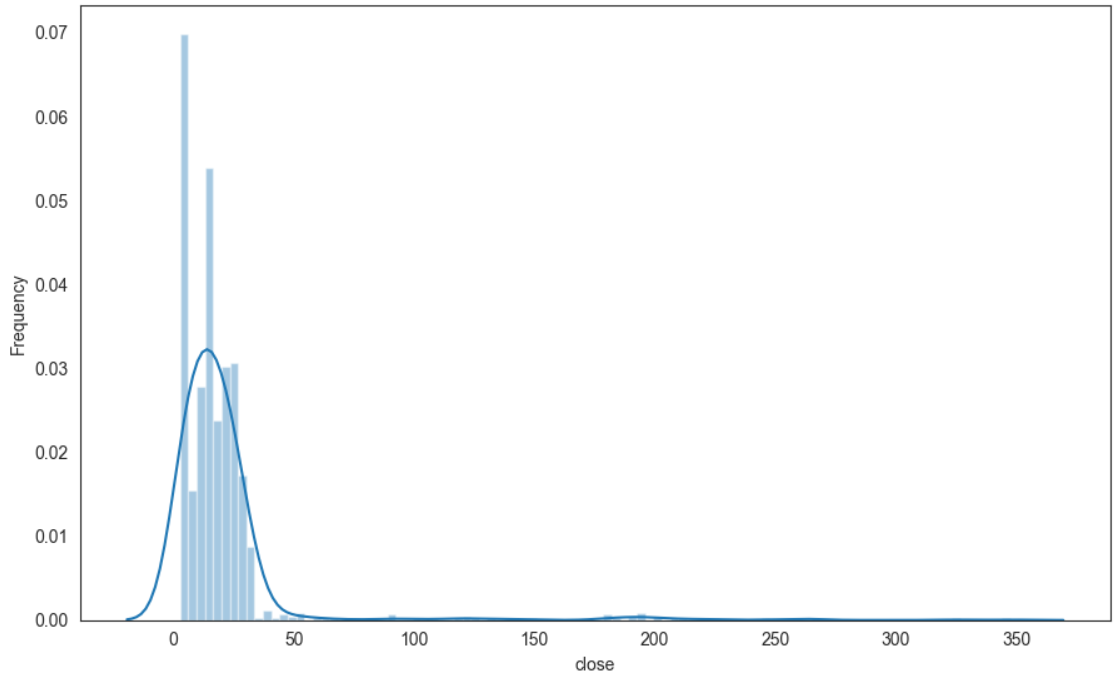
\includegraphics[width=15cm,height=7cm,keepaspectratio]{resultsEvaluation/closeDescMax.png}
\caption{Closing Prices with entire dataset}
\label{fig:appendix_closeDescMax}
\end{figure}
\begin{center}
\begin{tabular}{ c c }
\hline
\multicolumn{2}{|c|}{Closing Price Descriptive Statistics with entire dataset} \\
\hline
Mean & 20.25539316918189 \\
Standard Error & 0.8617871146224114 \\
Median & 15.22 \\
Mode & 4.14 \\
Standard Deviation & 30.56612021354625 \\
Sample Variance & 935.0303819398896 \\
Kurtosis & 43.00117239290764 \\
Skewness & 6.080884821536175 \\
Range & 344.71 \\
Minimum & 2.8 \\
Maximum & 347.51 \\
Sum & 25501.540000000005 \\
Count & 1259  
\end{tabular}
\end{center}

\subsubsection{Last Year}

\begin{figure}[h!]
\centering
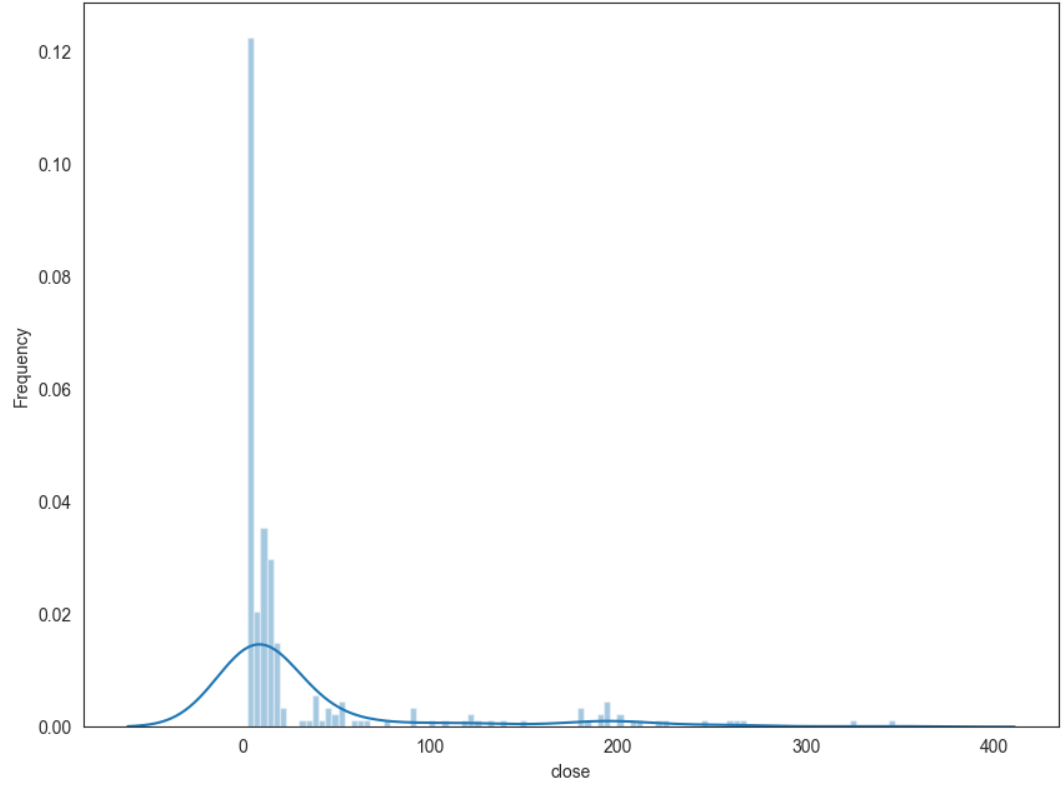
\includegraphics[width=15cm,height=7cm,keepaspectratio]{resultsEvaluation/closeDesc1.png}
\caption{Closing Prices in the last year of data}
\label{fig:appendix_closeDesc1}
\end{figure}
\begin{center}
\begin{tabular}{ c c }
\hline
\multicolumn{2}{|c|}{Closing Price Descriptive Statistics in the last year of data} \\
\hline
Mean & 35.32043478260869 \\
Standard Error & 4.034091200037088 \\
Median & 10.02 \\
Mode & 4.44 \\
Standard Deviation & 64.03921248871352 \\
Sample Variance & 4117.294627984817 \\
Kurtosis & 6.11122201031286 \\
Skewness & 2.5837008559997834 \\
Range & 344.71 \\
Minimum & 2.8 \\
Maximum & 347.51 \\
Sum & 8936.07 \\
Count & 253
\end{tabular}
\end{center}

\subsection{Trading Volume}

\subsubsection{Entire Dataset}

\begin{figure}[h!]
\centering
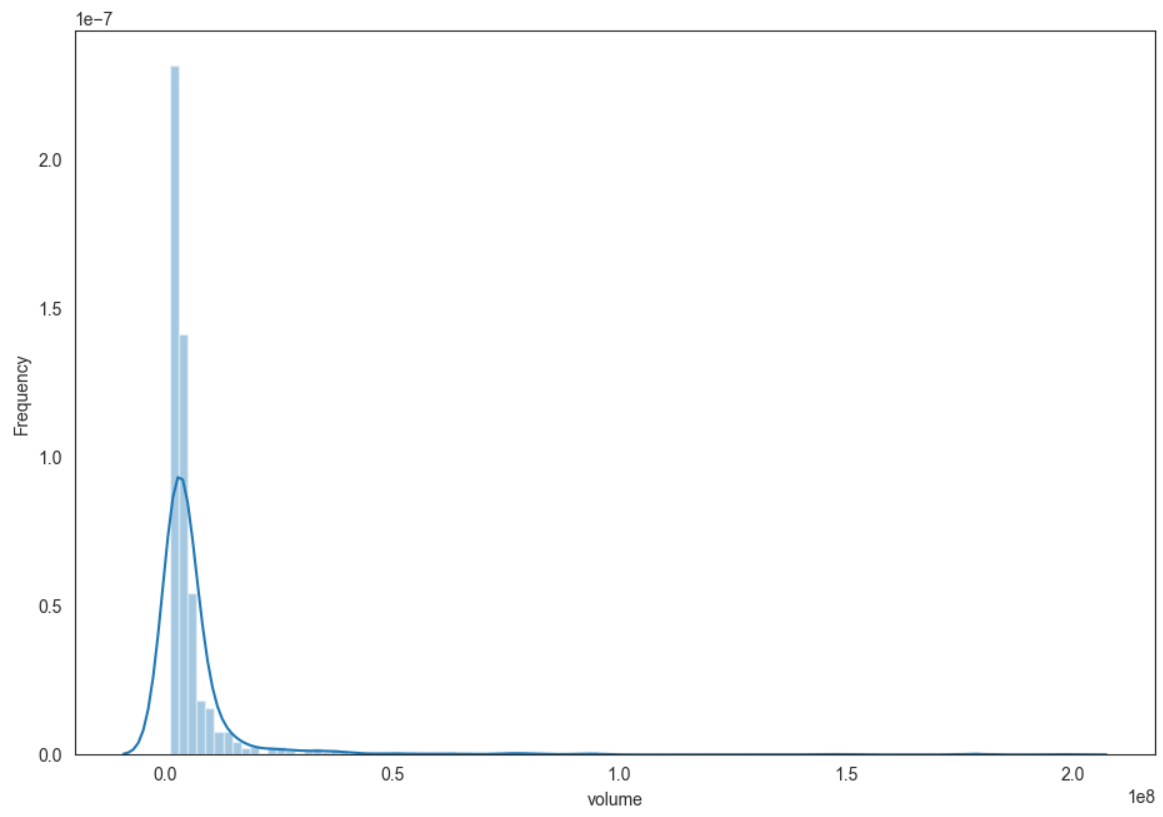
\includegraphics[width=15cm,height=7cm,keepaspectratio]{resultsEvaluation/volumeDescMax.png}
\caption{Trading Volume with entire dataset}
\label{fig:appendix_volumeDescMax}
\end{figure}
\begin{center}
\begin{tabular}{ c c }
\hline
\multicolumn{2}{|c|}{Trading Volume Descriptive Statistics with entire dataset} \\
\hline
Mean & 6435867.801429706 \\
Standard Error & 399372.9943423072 \\
Median & 3130713 \\
Mode & 1491760 \\
Standard Deviation & 14165079.458700724 \\
Sample Variance & 200808974859915.2 \\
Kurtosis & 81.30752829995787 \\
Skewness & 8.021781388564962 \\
Range & 196185042 \\
Minimum & 972904 \\
Maximum & 197157946 \\
Sum & 8102757562 \\
Count & 1259
\end{tabular}
\end{center}

\subsubsection{Last Year}

\begin{figure}[h!]
\centering
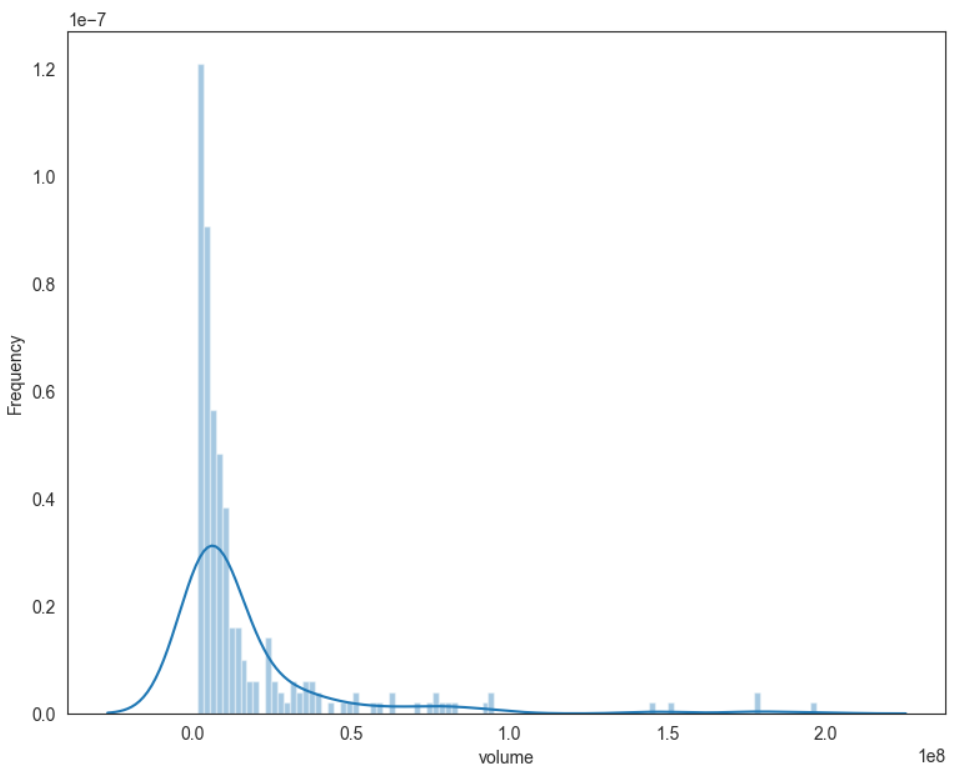
\includegraphics[width=15cm,height=7cm,keepaspectratio]{resultsEvaluation/volumeDesc1.png}
\caption{Trading Volume in the last year of data}
\label{fig:appendix_volumeDesc1}
\end{figure}
\begin{center}
\begin{tabular}{ c c }
\hline
\multicolumn{2}{|c|}{Trading Volume Descriptive Statistics in the last year of data} \\
\hline
Mean & 16731690.841897232 \\
Standard Error & 1798626.81876273 \\
Median & 6603951 \\
Mode & 4568695 \\
Standard Deviation & 28552315.58314456 \\
Sample Variance & 818469783592652.2 \\
Kurtosis & 16.215823114980463 \\
Skewness & 3.730320402302758 \\
Range & 195827485 \\
Minimum & 1330461 \\
Maximum & 197157946 \\
Sum & 4233117783 \\
Count & 253
\end{tabular}
\end{center}

\subsection{1 Day Returns}

\subsubsection{Entire Dataset}

\begin{figure}[h!]
\centering
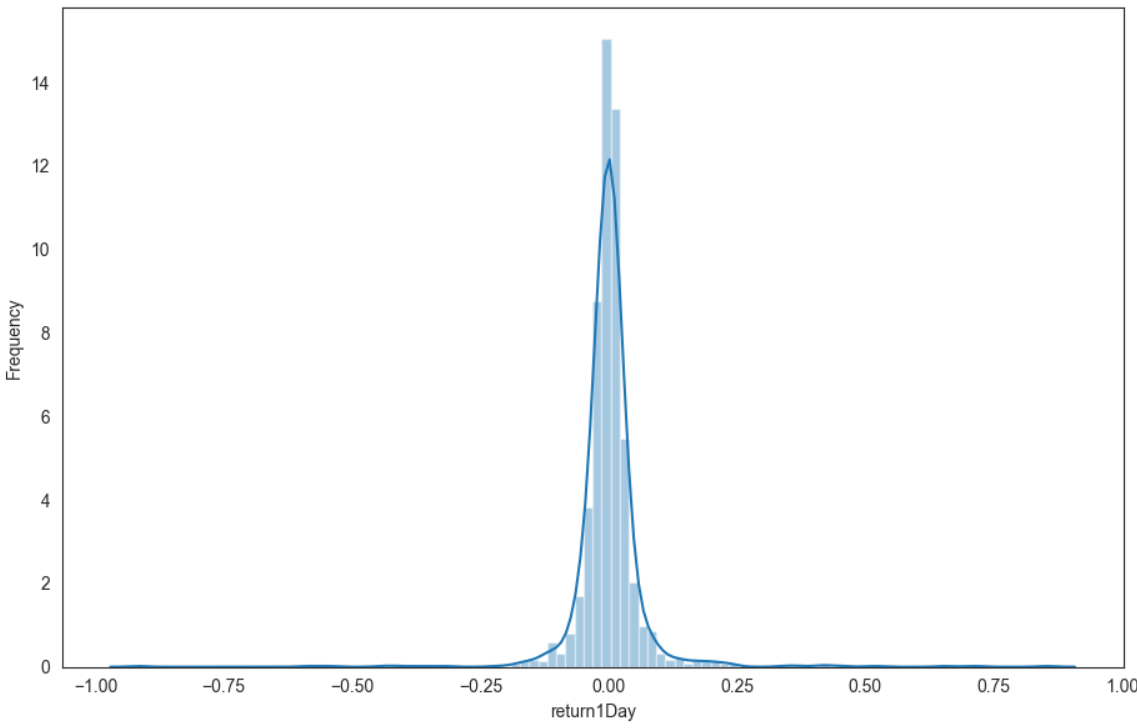
\includegraphics[width=15cm,height=7cm,keepaspectratio]{resultsEvaluation/1returnDescMax.png}
\caption{1 Day Returns with entire dataset}
\label{fig:appendix_1returnDescMax}
\end{figure}
\begin{center}
\begin{tabular}{ c c }
\hline
\multicolumn{2}{|c|}{1 Day Return Descriptive Statistics with entire dataset} \\
\hline
Mean & 0.0014490461774454091 \\
Standard Error & 0.0021291609999713954 \\
Median & 0.0 \\
Mode & 0.0 \\
Standard Deviation & 0.07548769098797223 \\
Sample Variance & 0.005702924817259385 \\
Kurtosis & 51.56501043384626 \\
Skewness & 0.7637560467880287 \\
Range & 1.770007043945965 \\
Minimum & -0.916290731874155 \\
Maximum & 0.85371631207181 \\
Sum & 1.8229000912263227 \\
Count & 1258
\end{tabular}
\end{center}

\subsubsection{Last Year}

\begin{figure}[h!]
\centering
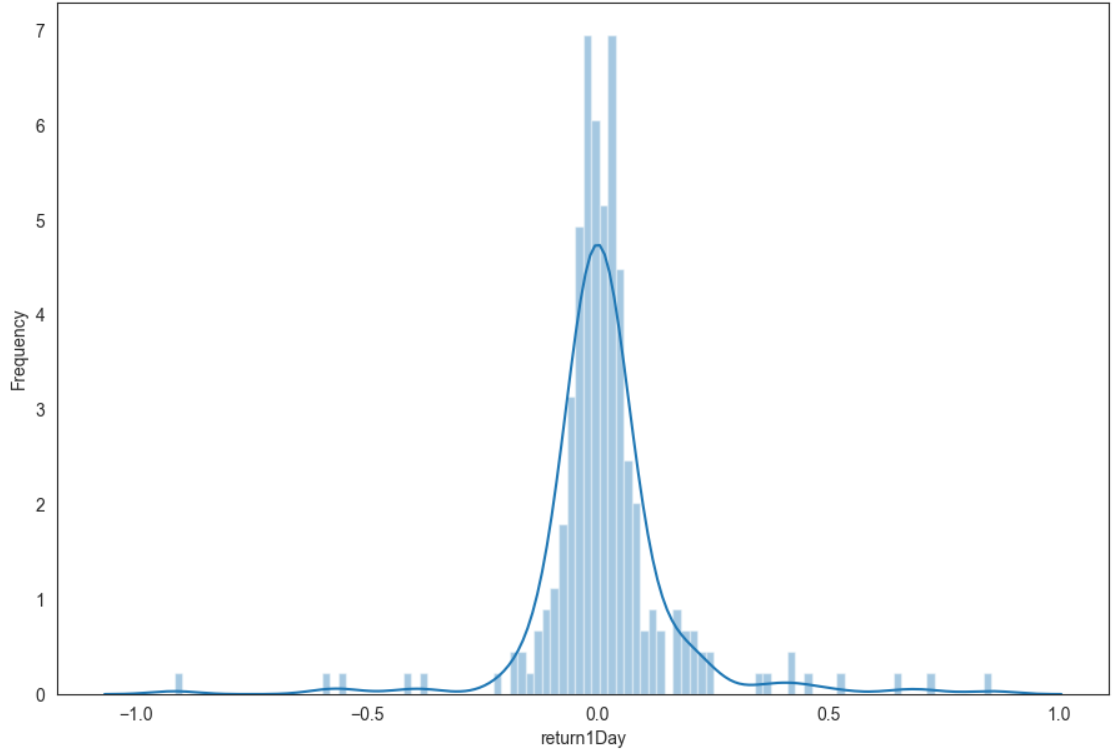
\includegraphics[width=15cm,height=7cm,keepaspectratio]{resultsEvaluation/1returnDesc1.png}
\caption{1 Day Returns in the last year of data}
\label{fig:appendix_1returnDesc1}
\end{figure}
\begin{center}
\begin{tabular}{ c c }
\hline
\multicolumn{2}{|c|}{1 Day Return Descriptive Statistics in the last year of data} \\
\hline
Mean & 0.01617449079992721 \\
Standard Error & 0.009609836418644279 \\
Median & 0.005313187705878563 \\
Mode & 0.022335953942063298 \\
Standard Deviation & 0.15224844154955602 \\
Sample Variance & 0.02327193691026168 \\
Kurtosis & 12.867982373920272 \\
Skewness & 0.32394336153811276 \\
Range & 1.770007043945965 \\
Minimum & -0.916290731874155 \\
Maximum & 0.85371631207181 \\
Sum & 4.075971681581655 \\
Count & 252
\end{tabular}
\end{center}

\subsection{Article Volume}

\subsubsection{Entire Dataset}

\begin{figure}[h!]
\centering
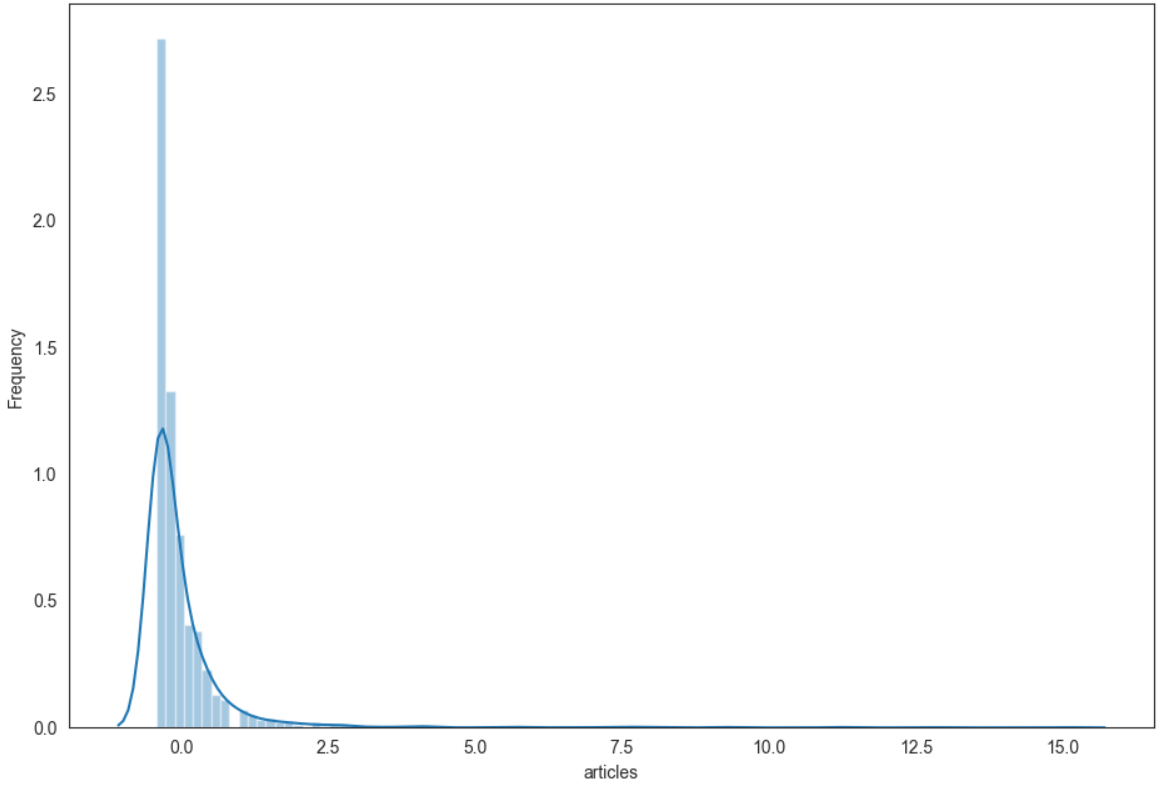
\includegraphics[width=15cm,height=7cm,keepaspectratio]{resultsEvaluation/articleDescMax.png}
\caption{Article Volume with entire dataset}
\label{fig:appendix_articleDescMax}
\end{figure}
\begin{center}
\begin{tabular}{ c c }
\hline
\multicolumn{2}{|c|}{Article Volume Descriptive Statistics with entire dataset} \\
\hline
Mean & -2.2065213996409285e-17 \\
Standard Error & 0.02196873875818734 \\
Median & -0.2421631034547878 \\
Mode & -0.41805802758295 \\
Standard Deviation & 1.0 \\
Sample Variance & 1.0004826254826256 \\
Kurtosis & 73.76924857053827 \\
Skewness & 7.360900854018193 \\
Range & 15.478753323278276 \\
Minimum & -0.41805802758295 \\
Maximum & 15.060695295695327 \\
Sum & -4.642022877199281e-12 \\
Count & 2073
\end{tabular}
\end{center}

\subsubsection{Last Year}

\begin{figure}[h!]
\centering
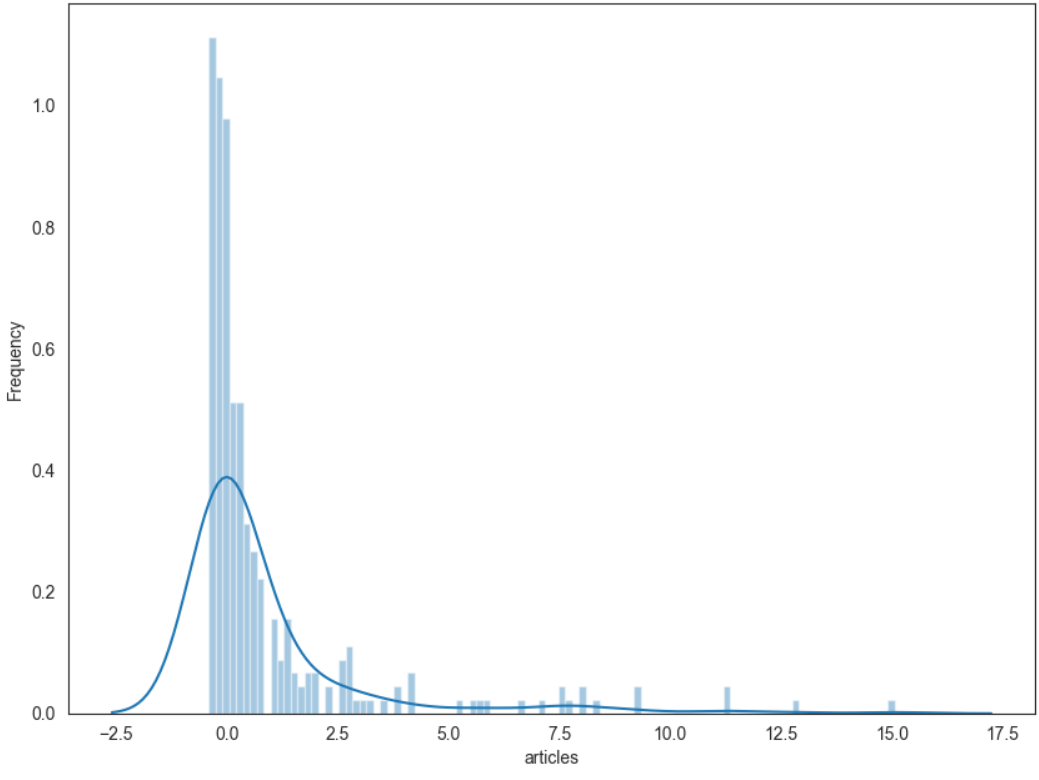
\includegraphics[width=15cm,height=7cm,keepaspectratio]{resultsEvaluation/articleDesc1.png}
\caption{Article Volume in the last year of data}
\label{fig:appendix_articleDesc1}
\end{figure}
\begin{center}
\begin{tabular}{ c c }
\hline
\multicolumn{2}{|c|}{Article Volume Descriptive Statistics in the last year of data} \\
\hline
Mean & 0.8623357132258448 \\
Standard Error & 0.1325148497318309 \\
Median & 0.1096267448015367 \\
Mode & -0.41805802758295 \\
Standard Deviation & 2.2527524454411254 \\
Sample Variance & 5.092453765840419 \\
Kurtosis & 12.21615870052046 \\
Skewness & 3.296079615884022 \\
Range & 15.478753323278276 \\
Minimum & -0.41805802758295 \\
Maximum & 15.060695295695327 \\
Sum & 250.07735683549507 \\
Count & 290
\end{tabular}
\end{center}

\subsection{Words Volume}

\subsubsection{Entire Dataset}

\begin{figure}[h!]
\centering
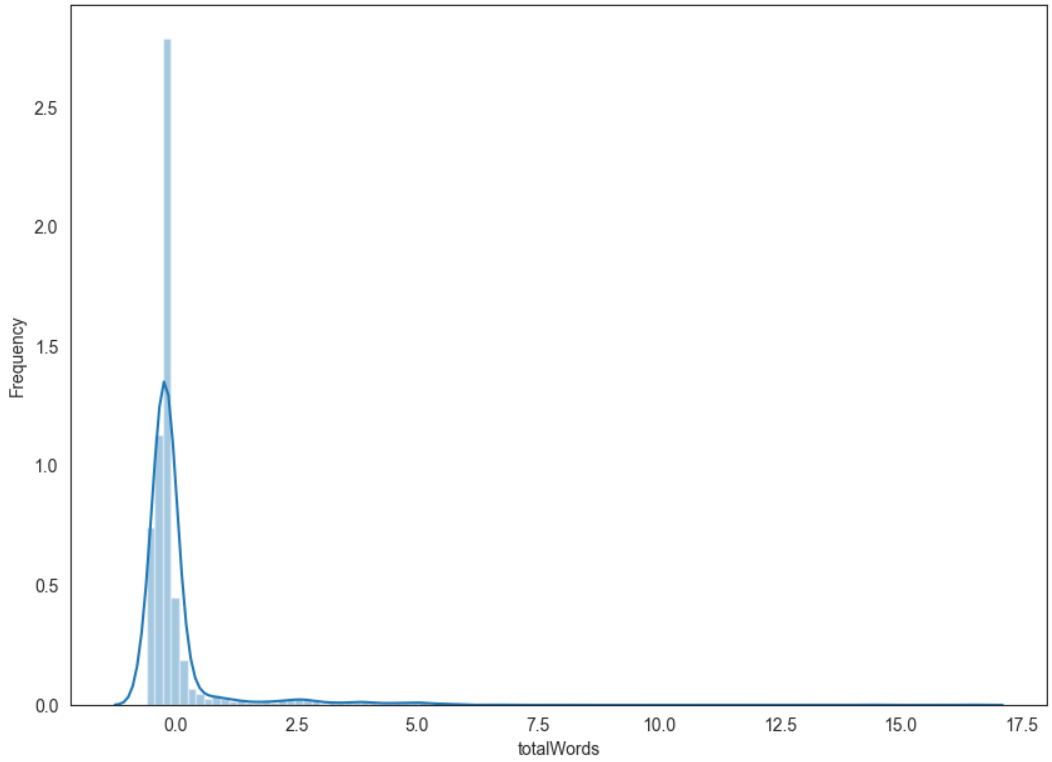
\includegraphics[width=15cm,height=7cm,keepaspectratio]{resultsEvaluation/wordsDescMax.png}
\caption{Words Volume with entire dataset}
\label{fig:appendix_wordsDescMax}
\end{figure}
\begin{center}
\begin{tabular}{ c c }
\hline
\multicolumn{2}{|c|}{Words Volume Descriptive Statistics with entire dataset} \\
\hline
Mean & 0.00013989387361311993 \\
Standard Error & 0.021968180574674083 \\
Median & -0.2 \\
Mode & -0.19 \\
Standard Deviation & 0.999974591918116 \\
Sample Variance & 1.0004317854395641 \\
Kurtosis & 66.70204164146547 \\
Skewness & 6.45609886055835 \\
Range & 17.07 \\
Minimum & -0.61 \\
Maximum & 16.46 \\
Sum & 0.28999999999995796 \\
Count & 2073
\end{tabular}
\end{center}

\subsubsection{Last Year}

\begin{figure}[h!]
\centering
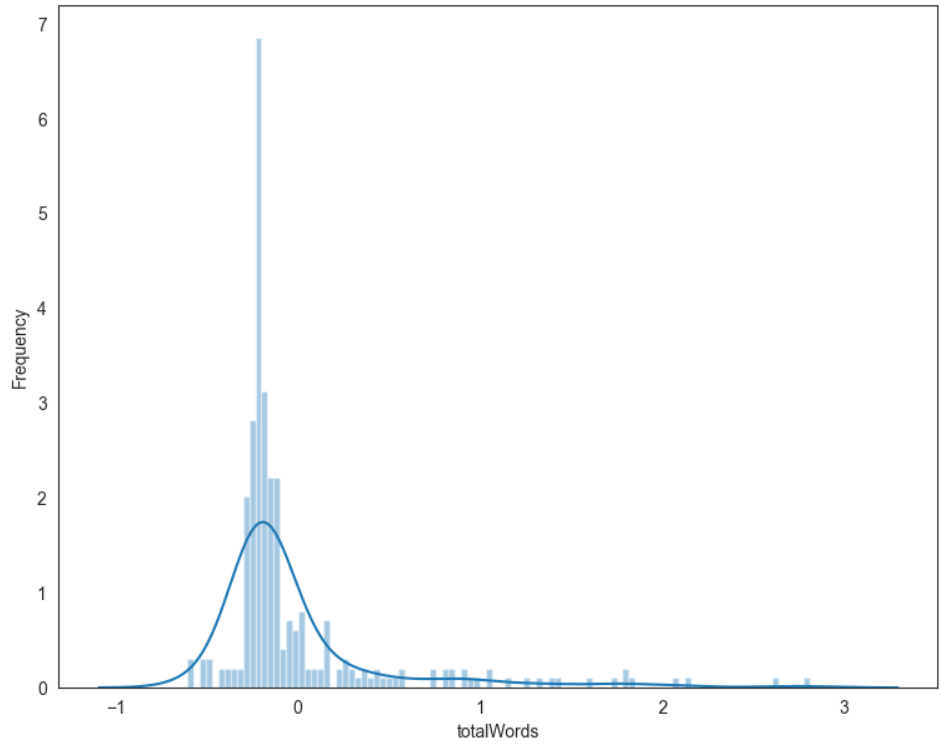
\includegraphics[width=15cm,height=7cm,keepaspectratio]{resultsEvaluation/wordsDesc1.png}
\caption{Words Volume in the last year of data}
\label{fig:appendix_wordsDesc1}
\end{figure}
\begin{center}
\begin{tabular}{ c c }
\hline
\multicolumn{2}{|c|}{Words Volume Descriptive Statistics in the last year of data} \\
\hline
Mean & -0.010758620689655175 \\
Standard Error & 0.029379055463608056 \\
Median & -0.19 \\
Mode & -0.22 \\
Standard Deviation & 0.4994439428813369 \\
Sample Variance & 0.2503073809807899 \\
Kurtosis & 9.61184972410166 \\
Skewness & 2.9411586965134755 \\
Range & 3.42 \\
Minimum & -0.61 \\
Maximum & 2.81 \\
Sum & -3.1200000000000068 \\
Count & 290
\end{tabular}
\end{center}

\subsection{Positive Sentiment}

\subsubsection{Entire Dataset}

\begin{figure}[h!]
\centering
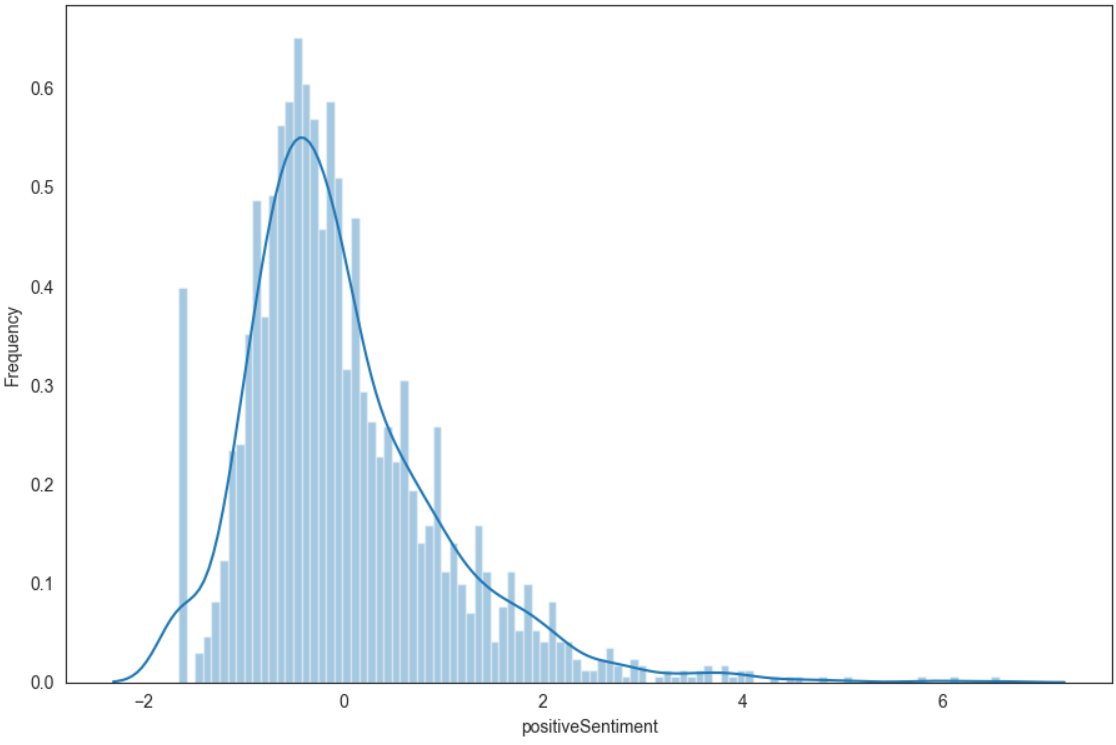
\includegraphics[width=15cm,height=7cm,keepaspectratio]{resultsEvaluation/positiveDescMax.png}
\caption{Positive Sentiment with entire dataset}
\label{fig:appendix_positiveDescMax}
\end{figure}
\begin{center}
\begin{tabular}{ c c }
\hline
\multicolumn{2}{|c|}{Positive Sentiment Descriptive Statistics with entire dataset} \\
\hline
Mean & -0.00011577424023154774 \\
Standard Error & 0.021969944580020426 \\
Median & -0.21 \\
Mode & -1.65 \\
Standard Deviation & 1.0000548880773885 \\
Sample Variance & 1.0005924576323273 \\
Kurtosis & 4.061676439612937 \\
Skewness & 1.4873401549309522 \\
Range & 8.22 \\
Minimum & -1.65 \\
Maximum & 6.57 \\
Sum & -0.23999999999965826 \\
Count & 2073
\end{tabular}
\end{center}

\subsubsection{Last Year}

\begin{figure}[h!]
\centering
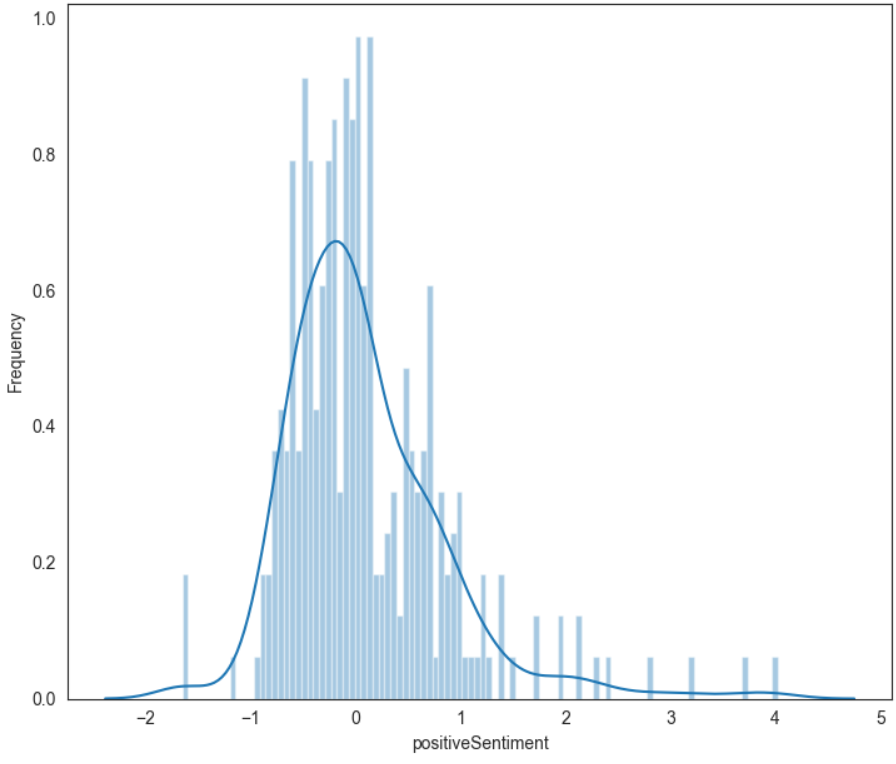
\includegraphics[width=15cm,height=7cm,keepaspectratio]{resultsEvaluation/positiveDesc1.png}
\caption{Positive Sentiment in the last year of data}
\label{fig:appendix_positiveDesc1}
\end{figure}
\begin{center}
\begin{tabular}{ c c }
\hline
\multicolumn{2}{|c|}{Positive Sentiment Descriptive Statistics in the last year of data} \\
\hline
Mean & 0.0863103448275862 \\
Standard Error & 0.04453127962901483 \\
Median & -0.055 \\
Mode & -0.1 \\
Standard Deviation & 0.7570317536932523 \\
Sample Variance & 0.5750801109652786 \\
Kurtosis & 5.009115638344465 \\
Skewness & 1.636685164397725 \\
Range & 5.67 \\
Minimum & -1.65 \\
Maximum & 4.02 \\
Sum & 25.029999999999973 \\
Count & 290
\end{tabular}
\end{center}

\subsection{Negative Sentiment}

\subsubsection{Entire Dataset}

\begin{figure}[h!]
\centering
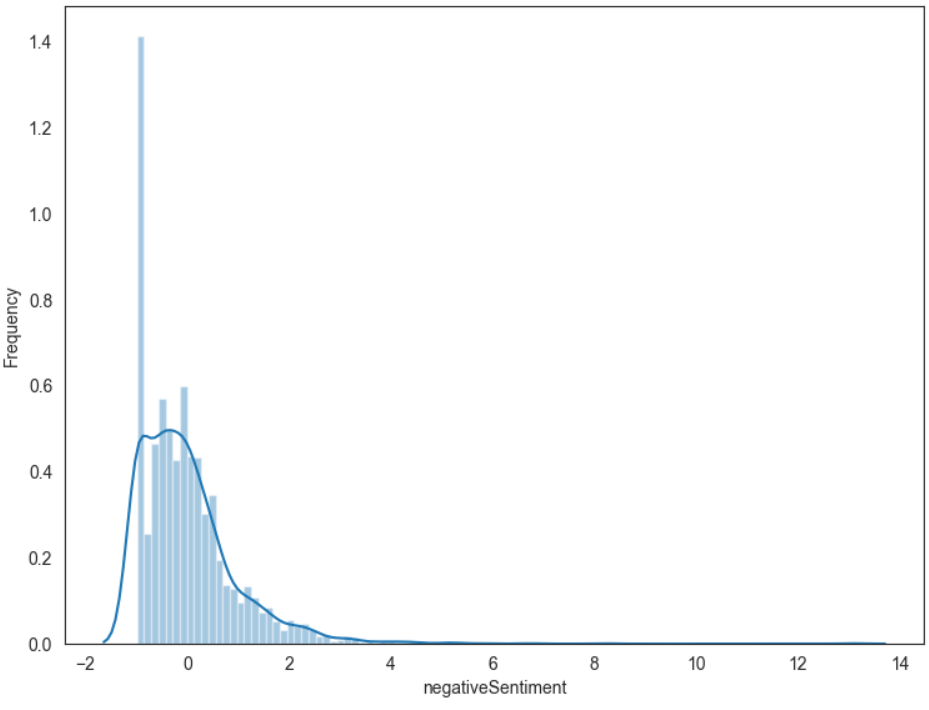
\includegraphics[width=15cm,height=7cm,keepaspectratio]{resultsEvaluation/negativeDescMax.png}
\caption{Negative Sentiment with entire dataset}
\label{fig:appendix_negativeDescMax}
\end{figure}
\begin{center}
\begin{tabular}{ c c }
\hline
\multicolumn{2}{|c|}{Negative Sentiment Descriptive Statistics with entire dataset} \\
\hline
Mean & 0.00014471780028943782 \\
Standard Error & 0.021964634770156394 \\
Median & -0.17 \\
Mode & -0.99 \\
Standard Deviation & 0.9998131896384166 \\
Sample Variance & 1.000108859355531 \\
Kurtosis & 19.513842113440127 \\
Skewness & 2.77912574439437 \\
Range & 14.05 \\
Minimum & -0.99 \\
Maximum & 13.06 \\
Sum & 0.30000000000174065 \\
Count & 2073
\end{tabular}
\end{center}

\subsubsection{Last Year}

\begin{figure}[h!]
\centering
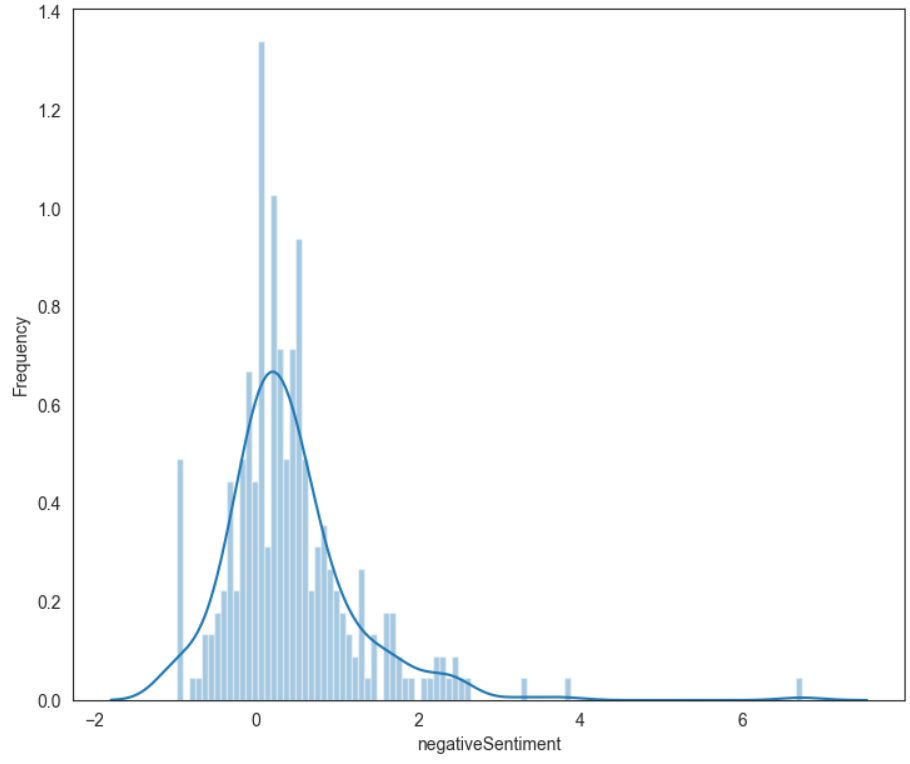
\includegraphics[width=15cm,height=7cm,keepaspectratio]{resultsEvaluation/negativeDesc1.png}
\caption{Negative Sentiment in the last year of data}
\label{fig:appendix_negativeDesc1}
\end{figure}
\begin{center}
\begin{tabular}{ c c }
\hline
\multicolumn{2}{|c|}{Negative Sentiment Descriptive Statistics in the last year of data} \\
\hline
Mean & 0.41293103448275864 \\
Standard Error & 0.04888104930864328 \\
Median & 0.27 \\
Mode & 0.08 \\
Standard Deviation & 0.8309778382469358 \\
Sample Variance & 0.6929135246390645 \\
Kurtosis & 11.895721323794636 \\
Skewness & 2.2637110757731076 \\
Range & 7.720000000000001 \\
Minimum & -0.99 \\
Maximum & 6.73 \\
Sum & 119.74999999999997 \\
Count & 290
\end{tabular}
\end{center}

\section{Auto-Correlation}
\label{appendix:autocorrelation}

\subsection{Closing Prices}

\begin{center}
\begin{tabular}{ c c c } 
\hline
\multicolumn{3}{|c|}{Closing Price AutoCorrelation with entire dataset} \\
\hline
Lag & Correlation & P-Value \\
\hline
1 & 0.9412 & 0.0 \\
2 & 0.9109 & 0.0 \\
3 & 0.8589 & 0.0 \\
4 & 0.7893 & 0.0 \\
5 & 0.7581 & 0.0 \\
\end{tabular}
\end{center}

\subsection{Trading Volume}

\begin{center}
\begin{tabular}{ c c c }
\hline
\multicolumn{3}{|c|}{Trading Volume AutoCorrelation with entire dataset} \\
\hline
Lag & Correlation & P-Value \\
\hline
1 & 0.7671 & 0.0 \\
2 & 0.6016 & 0.0 \\
3 & 0.5088 & 0.0 \\
4 & 0.4437 & 0.0 \\
5 & 0.4851 & 0.0 \\
\end{tabular}
\end{center}

\subsection{1 Day Returns}

\begin{center}
\begin{tabular}{ c c c }
\hline
\multicolumn{3}{|c|}{1 Day Return AutoCorrelation with entire dataset} \\
\hline
Lag & Correlation & P-Value \\
\hline
1 & 0.01 & 0.722 \\
2 & 0.1342 & 0.0 \\
3 & 0.1771 & 0.0 \\
4 & -0.2328 & 0.0 \\
5 & 0.0306 & 0.2795 \\
\end{tabular}
\end{center}

\subsection{Article Volume}

\begin{center}
\begin{tabular}{ c c c }
\hline
\multicolumn{3}{|c|}{Article Volume AutoCorrelation with entire dataset} \\
\hline
Lag & Correlation & P-Value \\
\hline
1 & 0.7087 & 0.0 \\
2 & 0.5052 & 0.0 \\
3 & 0.3913 & 0.0 \\
4 & 0.3588 & 0.0 \\
5 & 0.4346 & 0.0 \\
\end{tabular}
\end{center}

\subsection{Word Volume}

\begin{center}
\begin{tabular}{ c c c }
\hline
\multicolumn{3}{|c|}{Word Volume AutoCorrelation with entire dataset} \\
\hline
Lag & Correlation & P-Value \\
\hline
1 & 0.0512 & 0.0198 \\
2 & 0.0317 & 0.1497 \\
3 & 0.037 & 0.0927 \\
4 & 0.0106 & 0.6302 \\
5 & 0.0285 & 0.1947 \\
\end{tabular}
\end{center}

\subsection{Positive Sentiment}

\begin{center}
\begin{tabular}{ c c c }
\hline
\multicolumn{3}{|c|}{Positive Sentiment AutoCorrelation with entire dataset} \\
\hline
Lag & Correlation & P-Value \\
\hline
1 & 0.2189 & 0.0 \\
2 & 0.167 & 0.0 \\
3 & 0.1394 & 0.0 \\
4 & 0.1571 & 0.0 \\
5 & 0.1268 & 0.0 \\
\end{tabular}
\end{center}

\subsection{Negative Sentiment}

\begin{center}
\begin{tabular}{ c c c }
\hline
\multicolumn{3}{|c|}{Negative Sentiment AutoCorrelation with entire dataset} \\
\hline
Lag & Correlation & P-Value \\
\hline
1 & 0.1936 & 0.0 \\
2 & 0.1473 & 0.0 \\
3 & 0.1388 & 0.0 \\
4 & 0.1002 & 0.0 \\
5 & 0.1903 & 0.0 \\
\end{tabular}
\end{center}

\section{Return Vs Sentiment Correlation}
\label{appendix:returnSentimentCorrelation}

\subsection{1 Day Return Vs Negative Sentiment}

\begin{figure}[h!]
\centering
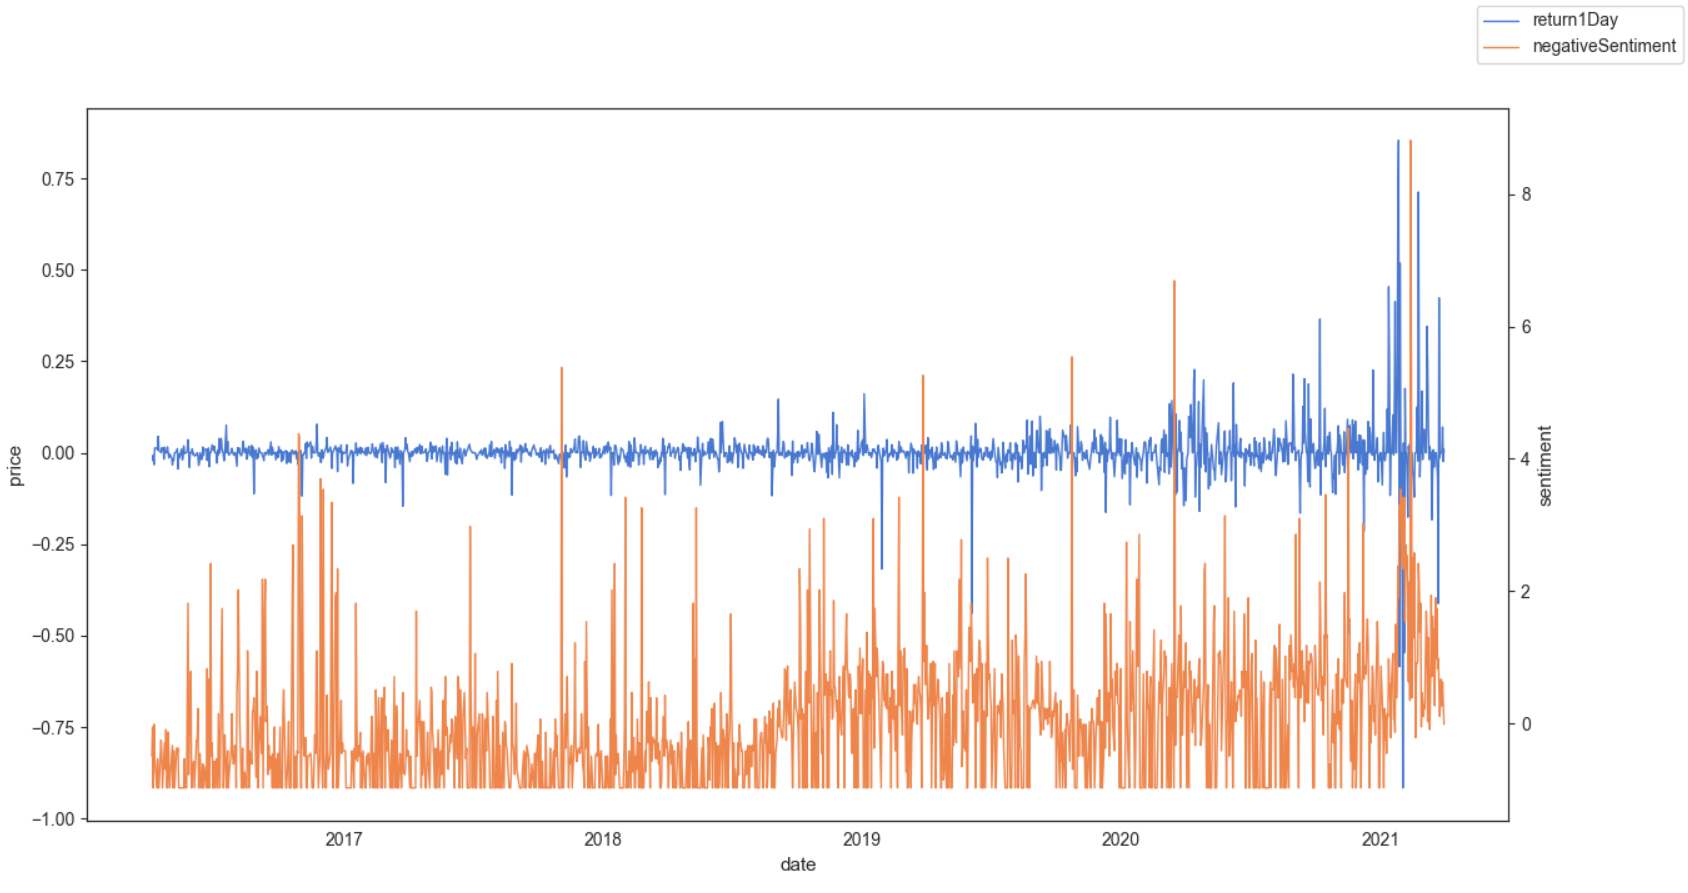
\includegraphics[width=15cm,height=7cm,keepaspectratio]{resultsEvaluation/1returnVsNeg.png}
\caption{1 Day Returns Vs Negative Sentiment with entire dataset}
\label{fig:appendix_1returnVsNeg}
\end{figure}

\begin{center}
\begin{tabular}{ c|c c|c c }
\hline
\multicolumn{5}{|c|}{1 Day Return Vs Negative Sentiment Correlation with entire dataset} \\
\hline
& \multicolumn{2}{|c|}{1 Day Return/Negative Sentiment} & \multicolumn{2}{|c }{Negative Sentiment/1 Day Return} \\
\hline
Lag & Correlation & P-Value & Correlation & P-Value \\
\hline
0 & -0.0057 & 0.8173 & -0.0057 & 0.8173 \\
1 & 0.0477 & 0.0554 & -0.0199 & 0.4249 \\
2 & 0.0318 & 0.2013 & -0.0186 & 0.4542 \\
3 & 0.0474 & 0.0571 & -0.0319 & 0.2002 \\
4 & -0.007 & 0.7782 & -0.0442 & 0.0757 \\
5 & 0.0431 & 0.0834 & -0.0444 & 0.0748 \\
\end{tabular}
\end{center}

\subsection{1 Day Return Vs Article Volume}

\begin{figure}[h!]
\centering
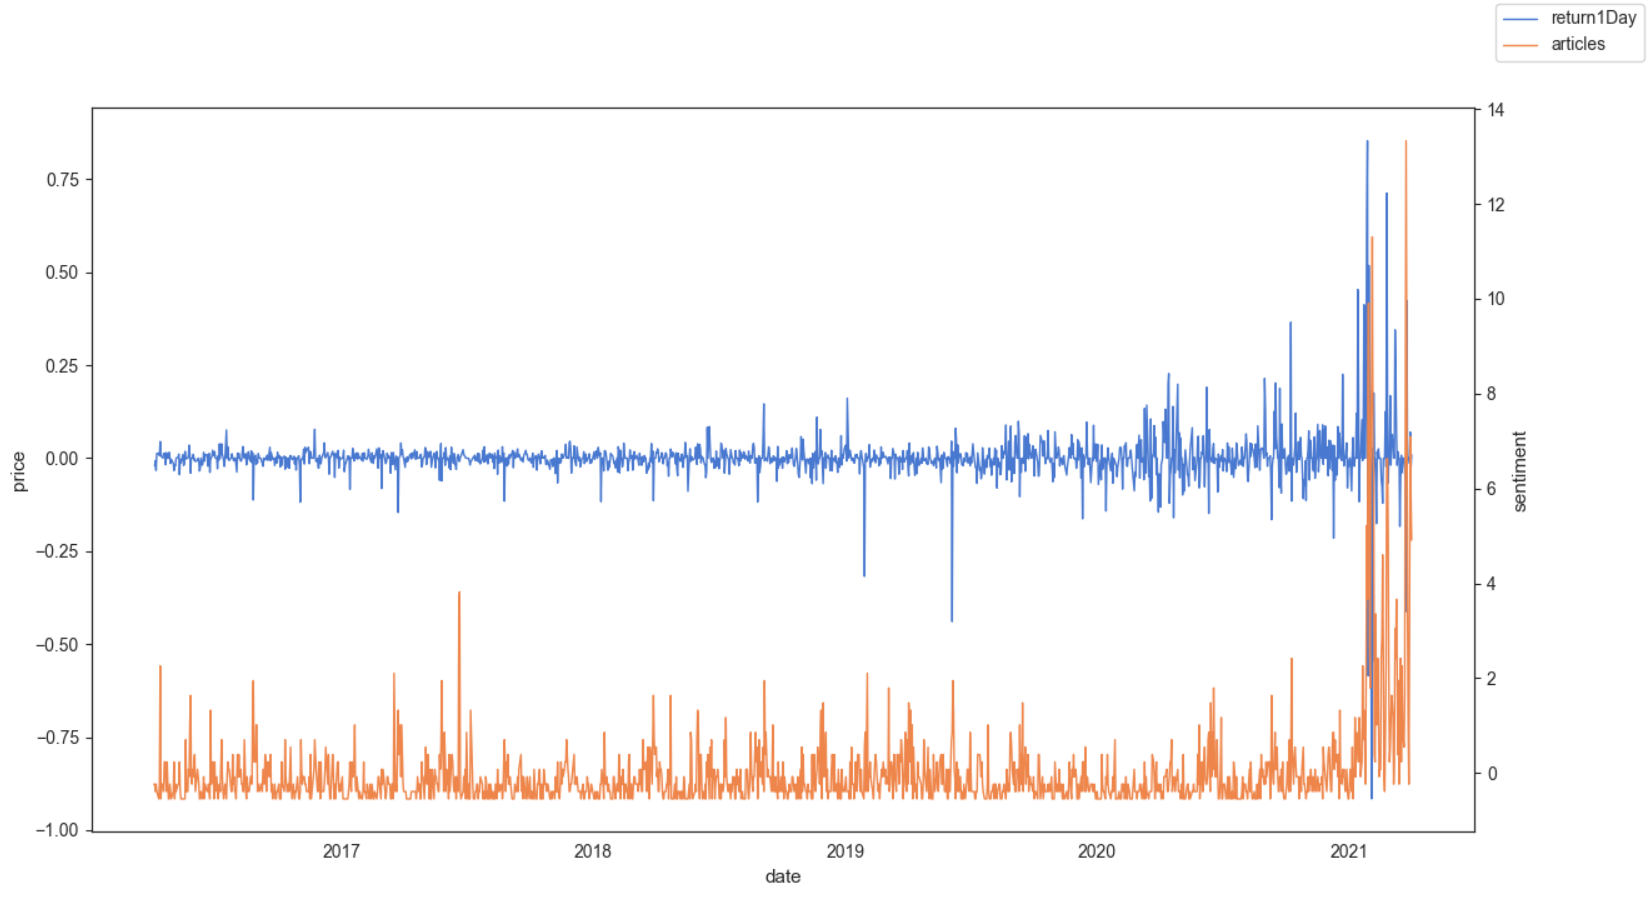
\includegraphics[width=15cm,height=7cm,keepaspectratio]{resultsEvaluation/1returnVsArticles.png}
\caption{1 Day Returns Vs Article Volume with entire dataset}
\label{fig:appendix_1returnVsArticle}
\end{figure}

\begin{center}
\begin{tabular}{ c|c c|c c }
\hline
\multicolumn{5}{|c|}{1 Day Return Vs Article Volume Correlation with entire dataset} \\
\hline
& \multicolumn{2}{|c|}{1 Day Return/Article Volume} & \multicolumn{2}{|c }{Article Volume/1 Day Return} \\
\hline
Lag & Correlation & P-Value & Correlation & P-Value \\
\hline
0 & -0.0316 & 0.2037 & -0.0316 & 0.2037 \\
1 & -0.0344 & 0.1674 & 0.019 & 0.4449 \\
2 & 0.0926 & 0.0002 & 0.0098 & 0.6924 \\
3 & 0.0749 & 0.0026 & -0.0354 & 0.1555 \\
4 & 0.0402 & 0.1066 & -0.07 & 0.0049 \\
5 & 0.1267 & 0.0 & -0.0679 & 0.0064 \\
\end{tabular}
\end{center}

\subsection{1 Day Return Vs Negative to Positive Sentiment Ratio}

\begin{figure}[h!]
\centering
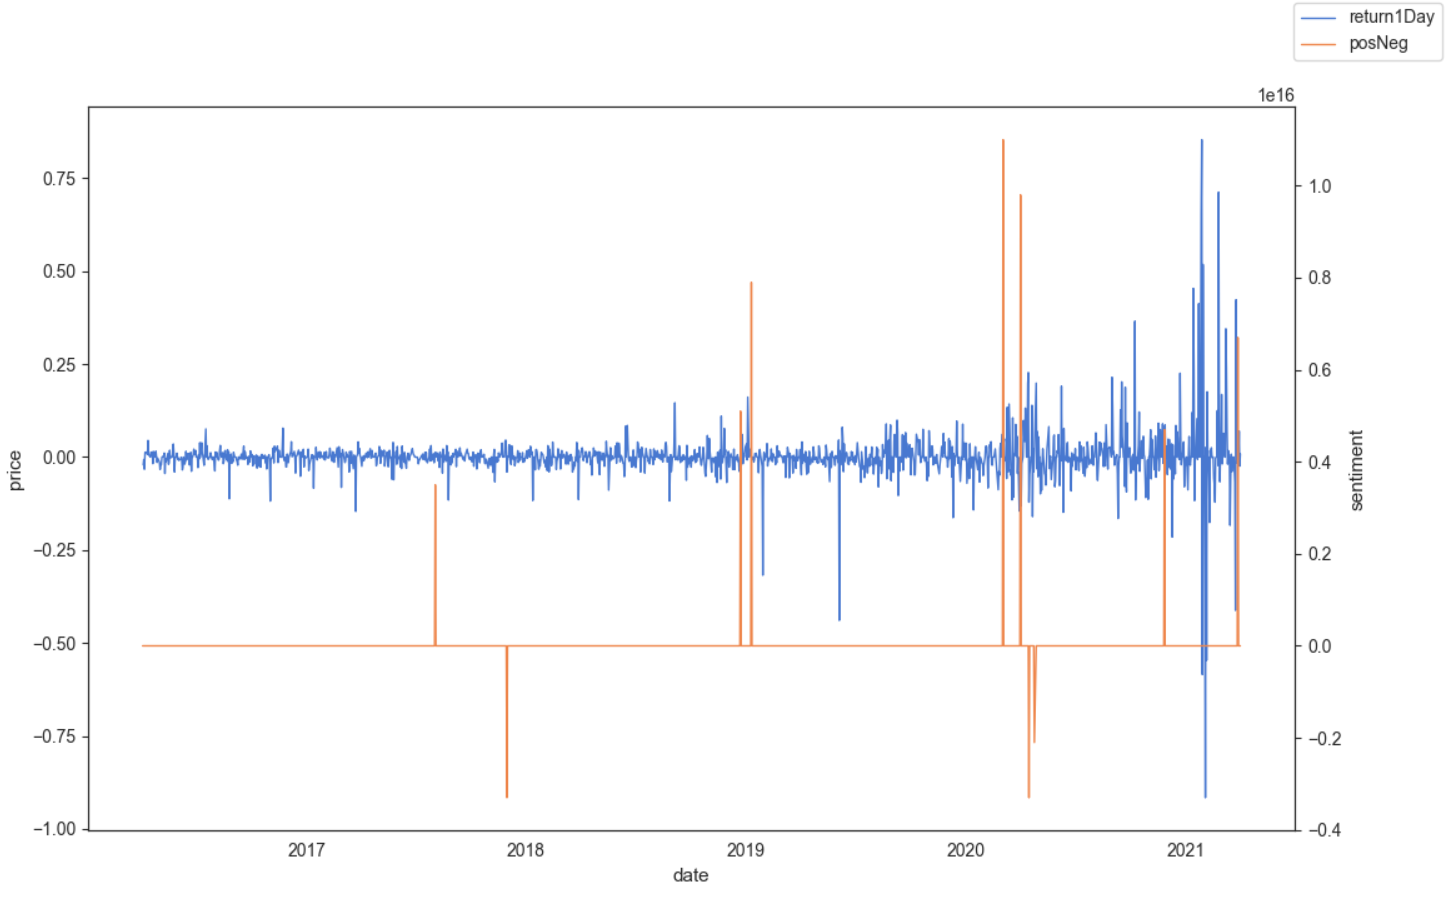
\includegraphics[width=15cm,height=7cm,keepaspectratio]{resultsEvaluation/1returnVsPosNeg.png}
\caption{1 Day Returns Vs Negative to Positive Sentiment Ratio with entire dataset}
\label{fig:appendix_1returnVsPosNeg}
\end{figure}

\begin{center}
\begin{tabular}{ c|c c|c c }
\hline
\multicolumn{5}{|c|}{1 Day Return Vs Negative to Positive Sentiment Ratio Correlation with entire dataset} \\
\hline
& \multicolumn{2}{|c|}{1 Day Return/Negative to Positive} & \multicolumn{2}{|c }{Negative to Positive/1 Day Return} \\
\hline
Lag & Correlation & P-Value & Correlation & P-Value \\
\hline
0 & -0.0152 & 0.5416 & -0.0152 & 0.5416 \\
1 & -0.0015 & 0.9513 & -0.0167 & 0.5031 \\
2 & -0.0476 & 0.0557 & 0.0177 & 0.4784 \\
3 & 0.0721 & 0.0038 & -0.0042 & 0.8674 \\
4 & -0.0615 & 0.0134 & 0.0187 & 0.4525 \\
5 & 0.0071 & 0.7761 & -0.0168 & 0.4997 \\
\end{tabular}
\end{center}

\section{Vector Autoregression}
\label{appendix:vectorAutoregression}

\subsection{1 Day Return and Negative Sentiment}

\subsubsection{Lag Selection}

\begin{center}
\begin{tabular}{ c c c c c c }
lags & loglik & p(LR) & AIC & BIC & HQC \\
\hline
1 & -117.24868 & & 0.153390 & 0.173485 & 0.160850 \\
2 & -83.29973 & 0.00000 & 0.116117 & 0.149608 & 0.128551 \\
3 & -73.30921 & 0.00050 & 0.108661 & 0.155550 & 0.126069 \\
4 & -52.32948 & 0.00000 & 0.087529 & 0.147814 & 0.109910 \\
5 & -23.21221 & 0.00000 & 0.056269 & 0.129951 & 0.083624 \\
6 & 33.11379 & 0.00000 & -0.008854 & 0.078225 & 0.023475 \\
7 & 35.69730 & 0.27059 & -0.007091 & 0.093385 & 0.030211 \\
8 & 45.00797 & 0.00093 & -0.013700 & 0.100172 & 0.028575 \\
\arrayrulecolor{red}\hline
9 & 49.69306 & 0.05248 & -0.014553 & 0.112716 & 0.032696 \\
\arrayrulecolor{red}\hline
10 & 51.88213 & 0.35724 & -0.012299 & 0.128367 & 0.039923 \\
\end{tabular}
\end{center}

\subsubsection{Unit Root Test}

\paragraph{1 Day Return}

Augmented Dickey-Fuller test for return1Day
testing down from 8 lags, criterion AIC
sample size 1608
unit-root null hypothesis: a = 1

test with constant
including 8 lags of (1-L)return1Day
model: (1-L)y = b0 + (a-1)*y(-1) + ... + e
estimated value of (a - 1): -0.944131
test statistic: tau\_c(1) = -14.6599
asymptotic p-value 3.842e-034
1st-order autocorrelation coeff. for e: -0.003
lagged differences: F(8, 1598) = 21.197 [0.0000]

\paragraph{Negative Sentiment}

Augmented Dickey-Fuller test for negativeSentiment
testing down from 8 lags, criterion AIC
sample size 1610
unit-root null hypothesis: a = 1

test with constant 
including 7 lags of (1-L)negativeSentiment
model: (1-L)y = b0 + (a-1)*y(-1) + ... + e
estimated value of (a - 1): -0.313169
test statistic: tau\_c(1) = -8.24341
asymptotic p-value 9.545e-014
1st-order autocorrelation coeff. for e: -0.002
lagged differences: F(7, 1601) = 20.863 [0.0000]

\subsubsection{Vector Autoregression}

\begin{center}
VAR system, lag order 8\\
OLS estimates, observations 2016-04-15--2022-06-15 ($T=1609$)
\end{center}
\noindent
Log-likelihood = 46.9491\par
\noindent
Determinant of covariance matrix = 0.00323375\par
\noindent
AIC $= -0.0161$ \par
\noindent
BIC $= 0.0977$ \par
\noindent
HQC $= 0.0261$ \par
\noindent
Portmanteau test: LB(48) = 399.605, df = 160 [0.0000]\par
\begin{center}

Equation 1: return1Day\\

\vspace{1em}

\begin{tabular}{lr@{.}lr@{.}lr@{.}lr@{.}l}
    &
    \multicolumn{2}{c}{Coefficient} &
    \multicolumn{2}{c}{Std.\ Error} &
    \multicolumn{2}{c}{$t$-ratio} &
    \multicolumn{2}{c}{p-value} \\[1ex]
const &
    0&000987822 &
    0&00158973 &
        0&6214 &
        0&5344 \\
return1Day$_{t-1}$ &
    0&0588697 &
    0&0250364 &
        2&351 &
        0&0188 \\
return1Day$_{t-2}$ &
    0&117217 &
    0&0251214 &
        4&666 &
        0&0000 \\
return1Day$_{t-3}$ &
    0&00727102 &
    0&0244870 &
        0&2969 &
        0&7666 \\
return1Day$_{t-4}$ &
    0&0321519 &
    0&0243106 &
        1&323 &
        0&1862 \\
return1Day$_{t-5}$ &
    0&125891 &
    0&0242941 &
        5&182 &
        0&0000 \\
return1Day$_{t-6}$ &
    $-$0&250912 &
    0&0244974 &
        $-$10&24 &
        0&0000 \\
return1Day$_{t-7}$ &
    0&0300316 &
    0&0251173 &
        1&196 &
        0&2320 \\
return1Day$_{t-8}$ &
    0&00446900 &
    0&0253934 &
        0&1760 &
        0&8603 \\
negativeSentiment\_1 &
    $-$0&000570795 &
    0&00176169 &
        $-$0&3240 &
        0&7460 \\
negativeSentiment\_2 &
    $-$0&00146513 &
    0&00179837 &
        $-$0&8147 &
        0&4154 \\
negativeSentiment\_3 &
    $-$0&000745000 &
    0&00180272 &
        $-$0&4133 &
        0&6795 \\
negativeSentiment\_4 &
    $-$0&00261853 &
    0&00179040 &
        $-$1&463 &
        0&1438 \\
negativeSentiment\_5 &
    $-$0&00140985 &
    0&00178944 &
        $-$0&7879 &
        0&4309 \\
negativeSentiment\_6 &
    0&00214476 &
    0&00180030 &
        1&191 &
        0&2337 \\
negativeSentiment\_7 &
    $-$0&000698839 &
    0&00179663 &
        $-$0&3890 &
        0&6973 \\
negativeSentiment\_8 &
    0&00326075 &
    0&00175921 &
        1&854 &
        0&0640 \\
\end{tabular}

\vspace{1ex}
\begin{tabular}{lrlr}
Mean dependent var &  0.001119 & S.D. dependent var &  0.066753 \\
Sum squared resid &  6.462398 & S.E. of regression &  0.063713 \\
$R^2$ &  0.098089 & Adjusted $R^2$ &  0.089024 \\
$F(16, 1592)$ &  10.82126 & P-value($F$) &  8.07\textrm{e--27} \\
$\hat{\rho}$ &  0.000578 & Durbin--Watson &  1.998764 \\
\end{tabular}


\end{center}

\begin{center}
F-tests of zero restrictions\\[1em]
\begin{tabular}{lll}
All lags of return1Day & $F(8, 1592) = 20.2874$ & [0.0000]\\
All lags of negativeSentiment & $F(8, 1592) = 1.0975$ & [0.3619]\\
All vars, lag 8 & $F(2, 1592) = 1.72858$ & [0.1779]\\
\end{tabular}
\end{center}

\clearpage

\begin{center}

Equation 2: negativeSentiment\\

\vspace{1em}

\begin{tabular}{lr@{.}lr@{.}lr@{.}lr@{.}l}
    &
    \multicolumn{2}{c}{Coefficient} &
    \multicolumn{2}{c}{Std.\ Error} &
    \multicolumn{2}{c}{$t$-ratio} &
    \multicolumn{2}{c}{p-value} \\[1ex]
const &
    7&90245\textrm{e--005} &
    0&0225083 &
        0&003511 &
        0&9972 \\
return1Day$_{t-1}$ &
    0&799396 &
    0&354478 &
        2&255 &
        0&0243 \\
return1Day$_{t-2}$ &
    0&732989 &
    0&355682 &
        2&061 &
        0&0395 \\
return1Day$_{t-3}$ &
    0&404381 &
    0&346699 &
        1&166 &
        0&2436 \\
return1Day$_{t-4}$ &
    $-$0&374238 &
    0&344203 &
        $-$1&087 &
        0&2771 \\
return1Day$_{t-5}$ &
    0&482715 &
    0&343969 &
        1&403 &
        0&1607 \\
return1Day$_{t-6}$ &
    0&0975990 &
    0&346847 &
        0&2814 &
        0&7784 \\
return1Day$_{t-7}$ &
    $-$0&0575599 &
    0&355624 &
        $-$0&1619 &
        0&8714 \\
return1Day$_{t-8}$ &
    1&08066 &
    0&359532 &
        3&006 &
        0&0027 \\
negativeSentiment\_1 &
    0&208236 &
    0&0249430 &
        8&348 &
        0&0000 \\
negativeSentiment\_2 &
    0&0828018 &
    0&0254623 &
        3&252 &
        0&0012 \\
negativeSentiment\_3 &
    0&0307012 &
    0&0255238 &
        1&203 &
        0&2292 \\
negativeSentiment\_4 &
    0&105098 &
    0&0253494 &
        4&146 &
        0&0000 \\
negativeSentiment\_5 &
    0&117337 &
    0&0253358 &
        4&631 &
        0&0000 \\
negativeSentiment\_6 &
    0&0467817 &
    0&0254896 &
        1&835 &
        0&0666 \\
negativeSentiment\_7 &
    0&0332576 &
    0&0254376 &
        1&307 &
        0&1913 \\
negativeSentiment\_8 &
    0&0623372 &
    0&0249078 &
        2&503 &
        0&0124 \\
\end{tabular}

\vspace{1ex}
\begin{tabular}{lrlr}
Mean dependent var &  0.005382 & S.D. dependent var &  1.000916 \\
Sum squared resid &  1295.477 & S.E. of regression &  0.902077 \\
$R^2$ &  0.195829 & Adjusted $R^2$ &  0.187747 \\
$F(16, 1592)$ &  24.22991 & P-value($F$) &  2.17\textrm{e--64} \\
$\hat{\rho}$ &  0.000219 & Durbin--Watson &  1.999505 \\
\end{tabular}


\end{center}

\begin{center}
F-tests of zero restrictions\\[1em]
\begin{tabular}{lll}
All lags of return1Day & $F(8, 1592) = 3.09983$ & [0.0018]\\
All lags of negativeSentiment & $F(8, 1592) = 44.948$ & [0.0000]\\
All vars, lag 8 & $F(2, 1592) = 7.53276$ & [0.0006]\\
\end{tabular}
\end{center}

\clearpage


\noindent For the system as a whole ---\par
Null hypothesis: the longest lag is 7\par
Alternative hypothesis: the longest lag is 8\par
Likelihood ratio test: $\chi^2_{4}$ = 18.596 [0.0009]\par    

\subsection{1 Day Return and Article Volume}

\subsubsection{Lag Selection}

\begin{center}
\begin{tabular}{ c c c c c c }
lags & loglik & p(LR) & AIC & BIC & HQC \\
\hline
1 & 355.55334 & & -0.435038 & -0.414943 & -0.427578 \\
2 & 393.91940 & 0.00000 & -0.477809 & -0.444317 & -0.465375 \\
3 & 399.65306 & 0.02178 & -0.479966 & -0.433078 & -0.462559 \\
4 & 416.64785 & 0.00000 & -0.496139 & -0.435854 & -0.473758 \\
5 & 498.71888 & 0.00000 & -0.593303 & -0.519621 & -0.565948 \\
6 & 591.91582 & 0.00000 & -0.704313 & -0.617235 & -0.671985 \\
7 & 603.23522 & 0.00015 & -0.713423 & -0.612948 & -0.676121 \\
8 & 603.57482 & 0.95387 & -0.708867 & -0.594995 & -0.666592 \\
\arrayrulecolor{red}\hline
9 & 616.39529 & 0.00004 & -0.719845 & -0.592576 & -0.672596 \\
\arrayrulecolor{red}\hline
10 & 618.08708 & 0.49580 & -0.716972 & -0.576307 & -0.664750 \\
\end{tabular}
\end{center}

\subsubsection{Unit Root Test}

\paragraph{1 Day Return}

Augmented Dickey-Fuller test for return1Day
testing down from 9 lags, criterion AIC
sample size 1607
unit-root null hypothesis: a = 1

test with constant 
including 9 lags of (1-L)return1Day
model: (1-L)y = b0 + (a-1)*y(-1) + ... + e
estimated value of (a - 1): -0.985703
test statistic: tau\_c(1) = -14.3735
asymptotic p-value 2.87e-033
1st-order autocorrelation coeff. for e: 0.002
lagged differences: F(9, 1596) = 19.198 [0.0000]

\paragraph{Article Volume}

Augmented Dickey-Fuller test for articles
testing down from 9 lags, criterion AIC
sample size 1609
unit-root null hypothesis: a = 1

test with constant 
including 8 lags of (1-L)articles
model: (1-L)y = b0 + (a-1)*y(-1) + ... + e
estimated value of (a - 1): -0.153152
test statistic: tau\_c(1) = -6.45545
asymptotic p-value 8.907e-009
1st-order autocorrelation coeff. for e: 0.001
lagged differences: F(8, 1599) = 26.622 [0.0000]

\subsubsection{Vector Autoregression}

\begin{center}
VAR system, lag order 9\\
OLS estimates, observations 2016-04-18--2022-06-15 ($T=1608$)
\end{center}
\noindent
Log-likelihood = 617.755\par
\noindent
Determinant of covariance matrix = 0.00158986\par
\noindent
AIC $= -0.7211$ \par
\noindent
BIC $= -0.5939$ \par
\noindent
HQC $= -0.6739$ \par
\noindent
Portmanteau test: LB(48) = 505.855, df = 156 [0.0000]\par
\begin{center}

Equation 1: return1Day\\

\vspace{1em}

\begin{tabular}{lr@{.}lr@{.}lr@{.}lr@{.}l}
    &
    \multicolumn{2}{c}{Coefficient} &
    \multicolumn{2}{c}{Std.\ Error} &
    \multicolumn{2}{c}{$t$-ratio} &
    \multicolumn{2}{c}{p-value} \\[1ex]
const &
    0&00108782 &
    0&00158045 &
        0&6883 &
        0&4914 \\
return1Day$_{t-1}$ &
    0&0591637 &
    0&0250827 &
        2&359 &
        0&0185 \\
return1Day$_{t-2}$ &
    0&122909 &
    0&0251453 &
        4&888 &
        0&0000 \\
return1Day$_{t-3}$ &
    $-$0&0245893 &
    0&0257675 &
        $-$0&9543 &
        0&3401 \\
return1Day$_{t-4}$ &
    0&0342852 &
    0&0249822 &
        1&372 &
        0&1701 \\
return1Day$_{t-5}$ &
    0&129546 &
    0&0248566 &
        5&212 &
        0&0000 \\
return1Day$_{t-6}$ &
    $-$0&267219 &
    0&0251912 &
        $-$10&61 &
        0&0000 \\
return1Day$_{t-7}$ &
    0&0303273 &
    0&0260085 &
        1&166 &
        0&2438 \\
return1Day$_{t-8}$ &
    0&0115134 &
    0&0263921 &
        0&4362 &
        0&6627 \\
return1Day$_{t-9}$ &
    $-$0&0685212 &
    0&0265911 &
        $-$2&577 &
        0&0101 \\
articles$_{t-1}$ &
    0&00766581 &
    0&00247897 &
        3&092 &
        0&0020 \\
articles$_{t-2}$ &
    $-$0&000435273 &
    0&00289421 &
        $-$0&1504 &
        0&8805 \\
articles$_{t-3}$ &
    $-$0&00383832 &
    0&00286352 &
        $-$1&340 &
        0&1803 \\
articles$_{t-4}$ &
    0&00189756 &
    0&00284012 &
        0&6681 &
        0&5042 \\
articles$_{t-5}$ &
    $-$0&00608534 &
    0&00283780 &
        $-$2&144 &
        0&0322 \\
articles$_{t-6}$ &
    $-$0&00164996 &
    0&00282611 &
        $-$0&5838 &
        0&5594 \\
articles$_{t-7}$ &
    $-$0&000697022 &
    0&00286670 &
        $-$0&2431 &
        0&8079 \\
articles$_{t-8}$ &
    $-$0&00234650 &
    0&00284151 &
        $-$0&8258 &
        0&4090 \\
articles$_{t-9}$ &
    0&00512786 &
    0&00259083 &
        1&979 &
        0&0480 \\
\end{tabular}

\vspace{1ex}
\begin{tabular}{lrlr}
Mean dependent var &  0.001117 & S.D. dependent var &  0.066774 \\
Sum squared resid &  6.364034 & S.E. of regression &  0.063286 \\
$R^2$ &  0.111815 & Adjusted $R^2$ &  0.101754 \\
$F(18, 1589)$ &  11.11346 & P-value($F$) &  1.33\textrm{e--30} \\
$\hat{\rho}$ & $-$0.003284 & Durbin--Watson &  2.006407 \\
\end{tabular}


\end{center}

\begin{center}
F-tests of zero restrictions\\[1em]
\begin{tabular}{lll}
All lags of return1Day & $F(9, 1589) = 19.5768$ & [0.0000]\\
All lags of articles & $F(9, 1589) = 3.00166$ & [0.0015]\\
All vars, lag 9 & $F(2, 1589) = 5.60717$ & [0.0037]\\
\end{tabular}
\end{center}

\clearpage

\begin{center}

Equation 2: articles\\

\vspace{1em}

\begin{tabular}{lr@{.}lr@{.}lr@{.}lr@{.}l}
    &
    \multicolumn{2}{c}{Coefficient} &
    \multicolumn{2}{c}{Std.\ Error} &
    \multicolumn{2}{c}{$t$-ratio} &
    \multicolumn{2}{c}{p-value} \\[1ex]
const &
    $-$0&000666807 &
    0&0159719 &
        $-$0&04175 &
        0&9667 \\
return1Day$_{t-1}$ &
    0&216461 &
    0&253484 &
        0&8539 &
        0&3933 \\
return1Day$_{t-2}$ &
    1&87414 &
    0&254116 &
        7&375 &
        0&0000 \\
return1Day$_{t-3}$ &
    0&0851509 &
    0&260405 &
        0&3270 &
        0&7437 \\
return1Day$_{t-4}$ &
    $-$0&528434 &
    0&252468 &
        $-$2&093 &
        0&0365 \\
return1Day$_{t-5}$ &
    1&25754 &
    0&251199 &
        5&006 &
        0&0000 \\
return1Day$_{t-6}$ &
    0&567181 &
    0&254581 &
        2&228 &
        0&0260 \\
return1Day$_{t-7}$ &
    1&17170 &
    0&262840 &
        4&458 &
        0&0000 \\
return1Day$_{t-8}$ &
    0&0307484 &
    0&266717 &
        0&1153 &
        0&9082 \\
return1Day$_{t-9}$ &
    $-$0&340330 &
    0&268727 &
        $-$1&266 &
        0&2055 \\
articles$_{t-1}$ &
    0&594105 &
    0&0250523 &
        23&71 &
        0&0000 \\
articles$_{t-2}$ &
    0&00941176 &
    0&0292487 &
        0&3218 &
        0&7477 \\
articles$_{t-3}$ &
    $-$0&0330034 &
    0&0289385 &
        $-$1&140 &
        0&2543 \\
articles$_{t-4}$ &
    $-$0&0151086 &
    0&0287021 &
        $-$0&5264 &
        0&5987 \\
articles$_{t-5}$ &
    0&0971494 &
    0&0286786 &
        3&388 &
        0&0007 \\
articles$_{t-6}$ &
    0&203121 &
    0&0285605 &
        7&112 &
        0&0000 \\
articles$_{t-7}$ &
    0&0639955 &
    0&0289706 &
        2&209 &
        0&0273 \\
articles$_{t-8}$ &
    0&0280164 &
    0&0287161 &
        0&9756 &
        0&3294 \\
articles$_{t-9}$ &
    $-$0&0970051 &
    0&0261828 &
        $-$3&705 &
        0&0002 \\
\end{tabular}

\vspace{1ex}
\begin{tabular}{lrlr}
Mean dependent var &  0.000485 & S.D. dependent var &  1.001466 \\
Sum squared resid &  649.9577 & S.E. of regression &  0.639559 \\
$R^2$ &  0.596729 & Adjusted $R^2$ &  0.592161 \\
$F(18, 1589)$ &  130.6266 & P-value($F$) &  3.0\textrm{e--297} \\
$\hat{\rho}$ &  0.001956 & Durbin--Watson &  1.995999 \\
\end{tabular}


\end{center}

\begin{center}
F-tests of zero restrictions\\[1em]
\begin{tabular}{lll}
All lags of return1Day & $F(9, 1589) = 14.8106$ & [0.0000]\\
All lags of articles & $F(9, 1589) = 232.346$ & [0.0000]\\
All vars, lag 9 & $F(2, 1589) = 7.40886$ & [0.0006]\\
\end{tabular}
\end{center}

\clearpage


\noindent For the system as a whole ---\par
Null hypothesis: the longest lag is 8\par
Alternative hypothesis: the longest lag is 9\par
Likelihood ratio test: $\chi^2_{4}$ = 25.673 [0.0000]\par    

\subsection{1 Day Return and Negative to Positive Sentiment Ratio}

\subsubsection{Lag Selection}

\begin{center}
\begin{tabular}{ c c c c c c }
lags & loglik & p(LR) & AIC & BIC & HQC \\
\hline
1 & -54352.12691 & & 67.990152 & 68.010329 & 67.997645 \\
2 & -54337.60145 & 0.00001 & 67.976987 & 68.010616 & 67.989475 \\
3 & -54332.85854 & 0.05004 & 67.976058 & 68.023138 & 67.993541 \\
4 & -54329.87651 & 0.20185 & 67.977331 & 68.037862 & 67.999809 \\
5 & -54318.60522 & 0.00016 & 67.968237 & 68.042218 & 67.995709 \\
6 & -54263.68536 & 0.00000 & 67.904547 & 67.991980 & 67.937015 \\
7 & -54262.74750 & 0.75860 & 67.908377 & 68.009261 & 67.945840 \\
8 & -54262.15282 & 0.87985 & 67.912636 & 68.026972 & 67.955094 \\
9 & -54257.65291 & 0.06110 & 67.912011 & 68.039798 & 67.959464 \\
10 & -54253.59146 & 0.08718 & 67.911934 & 68.053172 & 67.964382 \\
11 & -54250.55534 & 0.19382 & 67.913140 & 68.067829 & 67.970583 \\
12 & -54239.28045 & 0.00016 & 67.904041 & 68.072181 & 67.966479 \\
13 & -54238.32026 & 0.75040 & 67.907843 & 68.089434 & 67.975276 \\
14 & -54235.68328 & 0.26032 & 67.909548 & 68.104591 & 67.981976 \\
15 & -54224.18774 & 0.00013 & 67.900172 & 68.108667 & 67.977596 \\
16 & -54221.31635 & 0.21920 & 67.901584 & 68.123529 & 67.984002 \\
17 & -54216.80810 & 0.06069 & 67.900948 & 68.136345 & 67.988362 \\
\arrayrulecolor{red}\hline
18 & -54211.37297 & 0.02806 & 67.899153 & 68.148001 & 67.991562 \\
\arrayrulecolor{red}\hline
\end{tabular}
\end{center}

\subsubsection{Unit Root Test}

\paragraph{1 Day Return}

Augmented Dickey-Fuller test for return1Day
testing down from 18 lags, criterion AIC
sample size 1598
unit-root null hypothesis: a = 1

test with constant 
including 18 lags of (1-L)return1Day
model: (1-L)y = b0 + (a-1)*y(-1) + ... + e
estimated value of (a - 1): -1.00513
test statistic: tau\_c(1) = -10.3946
asymptotic p-value 1.778e-020
1st-order autocorrelation coeff. for e: -0.008
lagged differences: F(18, 1578) = 11.544 [0.0000]

\paragraph{Negative to Positive Sentiment Ratio}

Augmented Dickey-Fuller test for posNeg
testing down from 18 lags, criterion AIC
sample size 1603
unit-root null hypothesis: a = 1

test with constant 
including 14 lags of (1-L)posNeg
model: (1-L)y = b0 + (a-1)*y(-1) + ... + e
estimated value of (a - 1): -0.985466
test statistic: tau\_c(1) = -9.56218
asymptotic p-value 8.259e-018
1st-order autocorrelation coeff. for e: 0.000
lagged differences: F(14, 1587) = 2.088 [0.0102]

\subsubsection{Vector Autoregression}

\begin{center}
VAR system, lag order 18\\
OLS estimates, observations 2016-04-29--2022-06-15 ($T=1599$)
\end{center}
\noindent
Log-likelihood = $-$54211.4\par
\noindent
Determinant of covariance matrix = 9.61793\textrm{e+026}\par
\noindent
AIC $= 67.8992$ \par
\noindent
BIC $= 68.1480$ \par
\noindent
HQC $= 67.9916$ \par
\noindent
Portmanteau test: LB(48) = 356.694, df = 120 [0.0000]\par
\begin{center}

Equation 1: return1Day\\

\vspace{1em}

\begin{tabular}{lr@{.}lr@{.}lr@{.}lr@{.}l}
    &
    \multicolumn{2}{c}{Coefficient} &
    \multicolumn{2}{c}{Std.\ Error} &
    \multicolumn{2}{c}{$t$-ratio} &
    \multicolumn{2}{c}{p-value} \\[1ex]
const &
    0&000878498 &
    0&00161400 &
        0&5443 &
        0&5863 \\
return1Day$_{t-1}$ &
    0&0688790 &
    0&0252360 &
        2&729 &
        0&0064 \\
return1Day$_{t-2}$ &
    0&120335 &
    0&0252255 &
        4&770 &
        0&0000 \\
return1Day$_{t-3}$ &
    $-$0&00220926 &
    0&0254116 &
        $-$0&08694 &
        0&9307 \\
return1Day$_{t-4}$ &
    0&0137453 &
    0&0254850 &
        0&5393 &
        0&5897 \\
return1Day$_{t-5}$ &
    0&147222 &
    0&0255322 &
        5&766 &
        0&0000 \\
return1Day$_{t-6}$ &
    $-$0&243889 &
    0&0258014 &
        $-$9&453 &
        0&0000 \\
return1Day$_{t-7}$ &
    0&0305939 &
    0&0264409 &
        1&157 &
        0&2474 \\
return1Day$_{t-8}$ &
    0&000915059 &
    0&0267384 &
        0&03422 &
        0&9727 \\
return1Day$_{t-9}$ &
    $-$0&0457966 &
    0&0271071 &
        $-$1&689 &
        0&0913 \\
return1Day$_{t-10}$ &
    $-$0&0767250 &
    0&0271049 &
        $-$2&831 &
        0&0047 \\
return1Day$_{t-11}$ &
    0&0596763 &
    0&0272050 &
        2&194 &
        0&0284 \\
return1Day$_{t-12}$ &
    0&0619307 &
    0&0272272 &
        2&275 &
        0&0231 \\
return1Day$_{t-13}$ &
    0&00711337 &
    0&0263977 &
        0&2695 &
        0&7876 \\
return1Day$_{t-14}$ &
    $-$0&0452466 &
    0&0261789 &
        $-$1&728 &
        0&0841 \\
return1Day$_{t-15}$ &
    0&0436626 &
    0&0262331 &
        1&664 &
        0&0962 \\
return1Day$_{t-16}$ &
    $-$0&0424864 &
    0&0262612 &
        $-$1&618 &
        0&1059 \\
return1Day$_{t-17}$ &
    0&0268009 &
    0&0260795 &
        1&028 &
        0&3043 \\
return1Day$_{t-18}$ &
    $-$0&0493069 &
    0&0260318 &
        $-$1&894 &
        0&0584 \\
posNeg$_{t-1}$ &
    0&000000 &
    0&000000 &
        $-$0&09467 &
        0&9246 \\
posNeg$_{t-2}$ &
    0&000000 &
    0&000000 &
        $-$0&5480 &
        0&5838 \\
posNeg$_{t-3}$ &
    0&000000 &
    0&000000 &
        1&322 &
        0&1862 \\
posNeg$_{t-4}$ &
    0&000000 &
    0&000000 &
        $-$0&1188 &
        0&9054 \\
posNeg$_{t-5}$ &
    0&000000 &
    0&000000 &
        $-$0&2157 &
        0&8292 \\
posNeg$_{t-6}$ &
    0&000000 &
    0&000000 &
        1&756 &
        0&0793 \\
posNeg$_{t-7}$ &
    0&000000 &
    0&000000 &
        0&5835 &
        0&5596 \\
posNeg$_{t-8}$ &
    0&000000 &
    0&000000 &
        $-$0&2431 &
        0&8080 \\
posNeg$_{t-9}$ &
    0&000000 &
    0&000000 &
        1&171 &
        0&2417 \\
posNeg$_{t-10}$ &
    0&000000 &
    0&000000 &
        1&374 &
        0&1695 \\
posNeg$_{t-11}$ &
    0&000000 &
    0&000000 &
        0&7281 &
        0&4667 \\
posNeg$_{t-12}$ &
    0&000000 &
    0&000000 &
        $-$1&888 &
        0&0592 \\
posNeg$_{t-13}$ &
    0&000000 &
    0&000000 &
        0&4501 &
        0&6527 \\
posNeg$_{t-14}$ &
    0&000000 &
    0&000000 &
        $-$1&248 &
        0&2123 \\
posNeg$_{t-15}$ &
    0&000000 &
    0&000000 &
        0&05418 &
        0&9568 \\
posNeg$_{t-16}$ &
    0&000000 &
    0&000000 &
        $-$1&564 &
        0&1179 \\
posNeg$_{t-17}$ &
    0&000000 &
    0&000000 &
        2&833 &
        0&0047 \\
posNeg$_{t-18}$ &
    0&000000 &
    0&000000 &
        $-$2&327 &
        0&0201 \\
\end{tabular}

\vspace{1ex}
\begin{tabular}{lrlr}
Mean dependent var &  0.001103 & S.D. dependent var &  0.066957 \\
Sum squared resid &  6.239384 & S.E. of regression &  0.063202 \\
$R^2$ &  0.129103 & Adjusted $R^2$ &  0.109031 \\
$F(36, 1562)$ &  6.432046 & P-value($F$) &  5.98\textrm{e--28} \\
$\hat{\rho}$ & $-$0.001199 & Durbin--Watson &  2.002309 \\
\end{tabular}


\end{center}

\begin{center}
F-tests of zero restrictions\\[1em]
\begin{tabular}{lll}
All lags of return1Day & $F(18, 1562) = 11.2863$ & [0.0000]\\
All lags of posNeg & $F(18, 1562) = 1.69326$ & [0.0343]\\
All vars, lag 18 & $F(2, 1562) = 4.47767$ & [0.0115]\\
\end{tabular}
\end{center}

\clearpage

\begin{center}

Equation 2: posNeg\\

\vspace{1em}

\begin{tabular}{lr@{.}lr@{.}lr@{.}lr@{.}l}
    &
    \multicolumn{2}{c}{Coefficient} &
    \multicolumn{2}{c}{Std.\ Error} &
    \multicolumn{2}{c}{$t$-ratio} &
    \multicolumn{2}{c}{p-value} \\[1ex]
const &
    2&50088\textrm{e+013} &
    1&28302\textrm{e+013} &
        1&949 &
        0&0514 \\
return1Day$_{t-1}$ &
    4&17721\textrm{e+013} &
    2&00609\textrm{e+014} &
        0&2082 &
        0&8351 \\
return1Day$_{t-2}$ &
    $-$3&52670\textrm{e+014} &
    2&00525\textrm{e+014} &
        $-$1&759 &
        0&0788 \\
return1Day$_{t-3}$ &
    6&70503\textrm{e+014} &
    2&02005\textrm{e+014} &
        3&319 &
        0&0009 \\
return1Day$_{t-4}$ &
    $-$5&95726\textrm{e+014} &
    2&02589\textrm{e+014} &
        $-$2&941 &
        0&0033 \\
return1Day$_{t-5}$ &
    8&94318\textrm{e+013} &
    2&02964\textrm{e+014} &
        0&4406 &
        0&6595 \\
return1Day$_{t-6}$ &
    $-$1&13872\textrm{e+014} &
    2&05104\textrm{e+014} &
        $-$0&5552 &
        0&5788 \\
return1Day$_{t-7}$ &
    3&33937\textrm{e+013} &
    2&10187\textrm{e+014} &
        0&1589 &
        0&8738 \\
return1Day$_{t-8}$ &
    $-$1&65358\textrm{e+014} &
    2&12553\textrm{e+014} &
        $-$0&7780 &
        0&4367 \\
return1Day$_{t-9}$ &
    3&07219\textrm{e+014} &
    2&15483\textrm{e+014} &
        1&426 &
        0&1541 \\
return1Day$_{t-10}$ &
    $-$3&80023\textrm{e+014} &
    2&15465\textrm{e+014} &
        $-$1&764 &
        0&0780 \\
return1Day$_{t-11}$ &
    2&50452\textrm{e+014} &
    2&16261\textrm{e+014} &
        1&158 &
        0&2470 \\
return1Day$_{t-12}$ &
    $-$8&74514\textrm{e+013} &
    2&16438\textrm{e+014} &
        $-$0&4040 &
        0&6862 \\
return1Day$_{t-13}$ &
    $-$3&40406\textrm{e+014} &
    2&09844\textrm{e+014} &
        $-$1&622 &
        0&1050 \\
return1Day$_{t-14}$ &
    $-$1&13429\textrm{e+014} &
    2&08104\textrm{e+014} &
        $-$0&5451 &
        0&5858 \\
return1Day$_{t-15}$ &
    2&39340\textrm{e+014} &
    2&08535\textrm{e+014} &
        1&148 &
        0&2513 \\
return1Day$_{t-16}$ &
    $-$9&58090\textrm{e+013} &
    2&08759\textrm{e+014} &
        $-$0&4589 &
        0&6463 \\
return1Day$_{t-17}$ &
    1&10601\textrm{e+013} &
    2&07314\textrm{e+014} &
        0&05335 &
        0&9575 \\
return1Day$_{t-18}$ &
    2&63233\textrm{e+014} &
    2&06935\textrm{e+014} &
        1&272 &
        0&2035 \\
posNeg$_{t-1}$ &
    0&00978987 &
    0&0252934 &
        0&3871 &
        0&6988 \\
posNeg$_{t-2}$ &
    $-$0&00871657 &
    0&0252944 &
        $-$0&3446 &
        0&7304 \\
posNeg$_{t-3}$ &
    0&0115141 &
    0&0252962 &
        0&4552 &
        0&6491 \\
posNeg$_{t-4}$ &
    $-$0&00625229 &
    0&0251473 &
        $-$0&2486 &
        0&8037 \\
posNeg$_{t-5}$ &
    $-$0&000673291 &
    0&0264898 &
        $-$0&02542 &
        0&9797 \\
posNeg$_{t-6}$ &
    $-$0&00615141 &
    0&0264904 &
        $-$0&2322 &
        0&8164 \\
posNeg$_{t-7}$ &
    $-$0&00263580 &
    0&0264151 &
        $-$0&09978 &
        0&9205 \\
posNeg$_{t-8}$ &
    0&000702172 &
    0&0264068 &
        0&02659 &
        0&9788 \\
posNeg$_{t-9}$ &
    0&0136048 &
    0&0263998 &
        0&5153 &
        0&6064 \\
posNeg$_{t-10}$ &
    0&000796289 &
    0&0264086 &
        0&03015 &
        0&9759 \\
posNeg$_{t-11}$ &
    $-$0&00343408 &
    0&0264175 &
        $-$0&1300 &
        0&8966 \\
posNeg$_{t-12}$ &
    $-$0&0908851 &
    0&0264172 &
        $-$3&440 &
        0&0006 \\
posNeg$_{t-13}$ &
    $-$0&00111835 &
    0&0265454 &
        $-$0&04213 &
        0&9664 \\
posNeg$_{t-14}$ &
    $-$0&00438177 &
    0&0265488 &
        $-$0&1650 &
        0&8689 \\
posNeg$_{t-15}$ &
    0&113097 &
    0&0265615 &
        4&258 &
        0&0000 \\
posNeg$_{t-16}$ &
    $-$0&00430047 &
    0&0267011 &
        $-$0&1611 &
        0&8721 \\
posNeg$_{t-17}$ &
    0&00221779 &
    0&0266895 &
        0&08310 &
        0&9338 \\
posNeg$_{t-18}$ &
    $-$0&00946776 &
    0&0267575 &
        $-$0&3538 &
        0&7235 \\
\end{tabular}

\vspace{1ex}
\begin{tabular}{lrlr}
Mean dependent var &  2.50\textrm{e+13} & S.D. dependent var &  5.06\textrm{e+14} \\
Sum squared resid &  3.94\textrm{e+32} & S.E. of regression &  5.02\textrm{e+14} \\
$R^2$ &  0.038065 & Adjusted $R^2$ &  0.015895 \\
$F(36, 1562)$ &  1.716939 & P-value($F$) &  0.005381 \\
$\hat{\rho}$ & $-$0.000284 & Durbin--Watson &  2.000563 \\
\end{tabular}


\end{center}

\begin{center}
F-tests of zero restrictions\\[1em]
\begin{tabular}{lll}
All lags of return1Day & $F(18, 1562) = 1.80018$ & [0.0206]\\
All lags of posNeg & $F(18, 1562) = 1.70901$ & [0.0318]\\
All vars, lag 18 & $F(2, 1562) = 0.874217$ & [0.4174]\\
\end{tabular}
\end{center}

\clearpage


\noindent For the system as a whole ---\par
Null hypothesis: the longest lag is 17\par
Alternative hypothesis: the longest lag is 18\par
Likelihood ratio test: $\chi^2_{4}$ = 10.870 [0.0281]\par    

TODO -
\subsection{1 Day Return, }

\subsubsection{Lag Selection}

\begin{center}
\begin{tabular}{ c c c c c c }
lags & loglik & p(LR) & AIC & BIC & HQC \\
\hline
\arrayrulecolor{red}\hline
\arrayrulecolor{red}\hline
\end{tabular}
\end{center}

\subsubsection{Unit Root Test}

\paragraph{1 Day Return}

\paragraph{}

\subsubsection{Vector Autoregression}
